\section{Task 1}
\begin{frame}[plain]
	\huge{Force \& Density Calculation}
\end{frame}

\subsection{Step 1: Density Verification}

\begin{frame}{Analytic Hernquist}

	Density distribution:
	\begin{equation}
		\rho(r) = \frac{M}{2\pi}\frac{a}{r}\frac{1}{(r+a)^3}
	\end{equation}

	Cumulative Mass distribution inside a radius:
	\begin{equation}
		M(r) = M \frac{r^2}{(r+a)^2}
		\label{eq:cumulative-mass-distribution}
	\end{equation}

	Reformed Half-mass-radius equation, to get scale length
	\begin{equation}
		a = \frac{r_{1/2}}{1+\sqrt 2}
	\end{equation}

	{\footnotesize Where:
	\begin{itemize}
		\item $M$  - Total mass of the system
		\item $a$ - Scale Length
		\item $r$ - Particle position vector
		\item $r_{1/2}$ - Half-mass radius: calculated numerically
	\end{itemize}}
\end{frame}

% since all particles have masses of 92. we assumed a mass of 1, to further simplify our equations
\begin{frame}{Numerical Density Approximation}
	Logarithmic binning via \texttt{Histogram} class into a \texttt{std::vector} of \texttt{Shell} classes.
	\begin{equation}
		i_{log} = |\vb{r}|_{min} (\frac{|\vb{r}|_{max}}{|\vb{r}|_{min}})^{\frac {i_{lin}}{n}}
	\end{equation}

	On histogram creation calculated for each shell:
	\begin{equation}
		\rho_i = M_i / V_i
	\end{equation}

	Poissonian density error with expected number of particles $\lambda = \frac{N}{B}$ and standard deviation
	$\sigma = \sqrt{\lambda}$:
	\begin{equation}
		\rho_{err} = \sigma \frac{m_p}{V_i}
	\end{equation}

	{\footnotesize
	Where:
	\begin{itemize}
		\item $i$ - Shell index
		\item $B$ - Number of bins in histogram
		\item $N$ - Number of Particles
		\item $m_p$ - Mass of a single particle
	\end{itemize}
	}
\end{frame}


\begin{frame}
	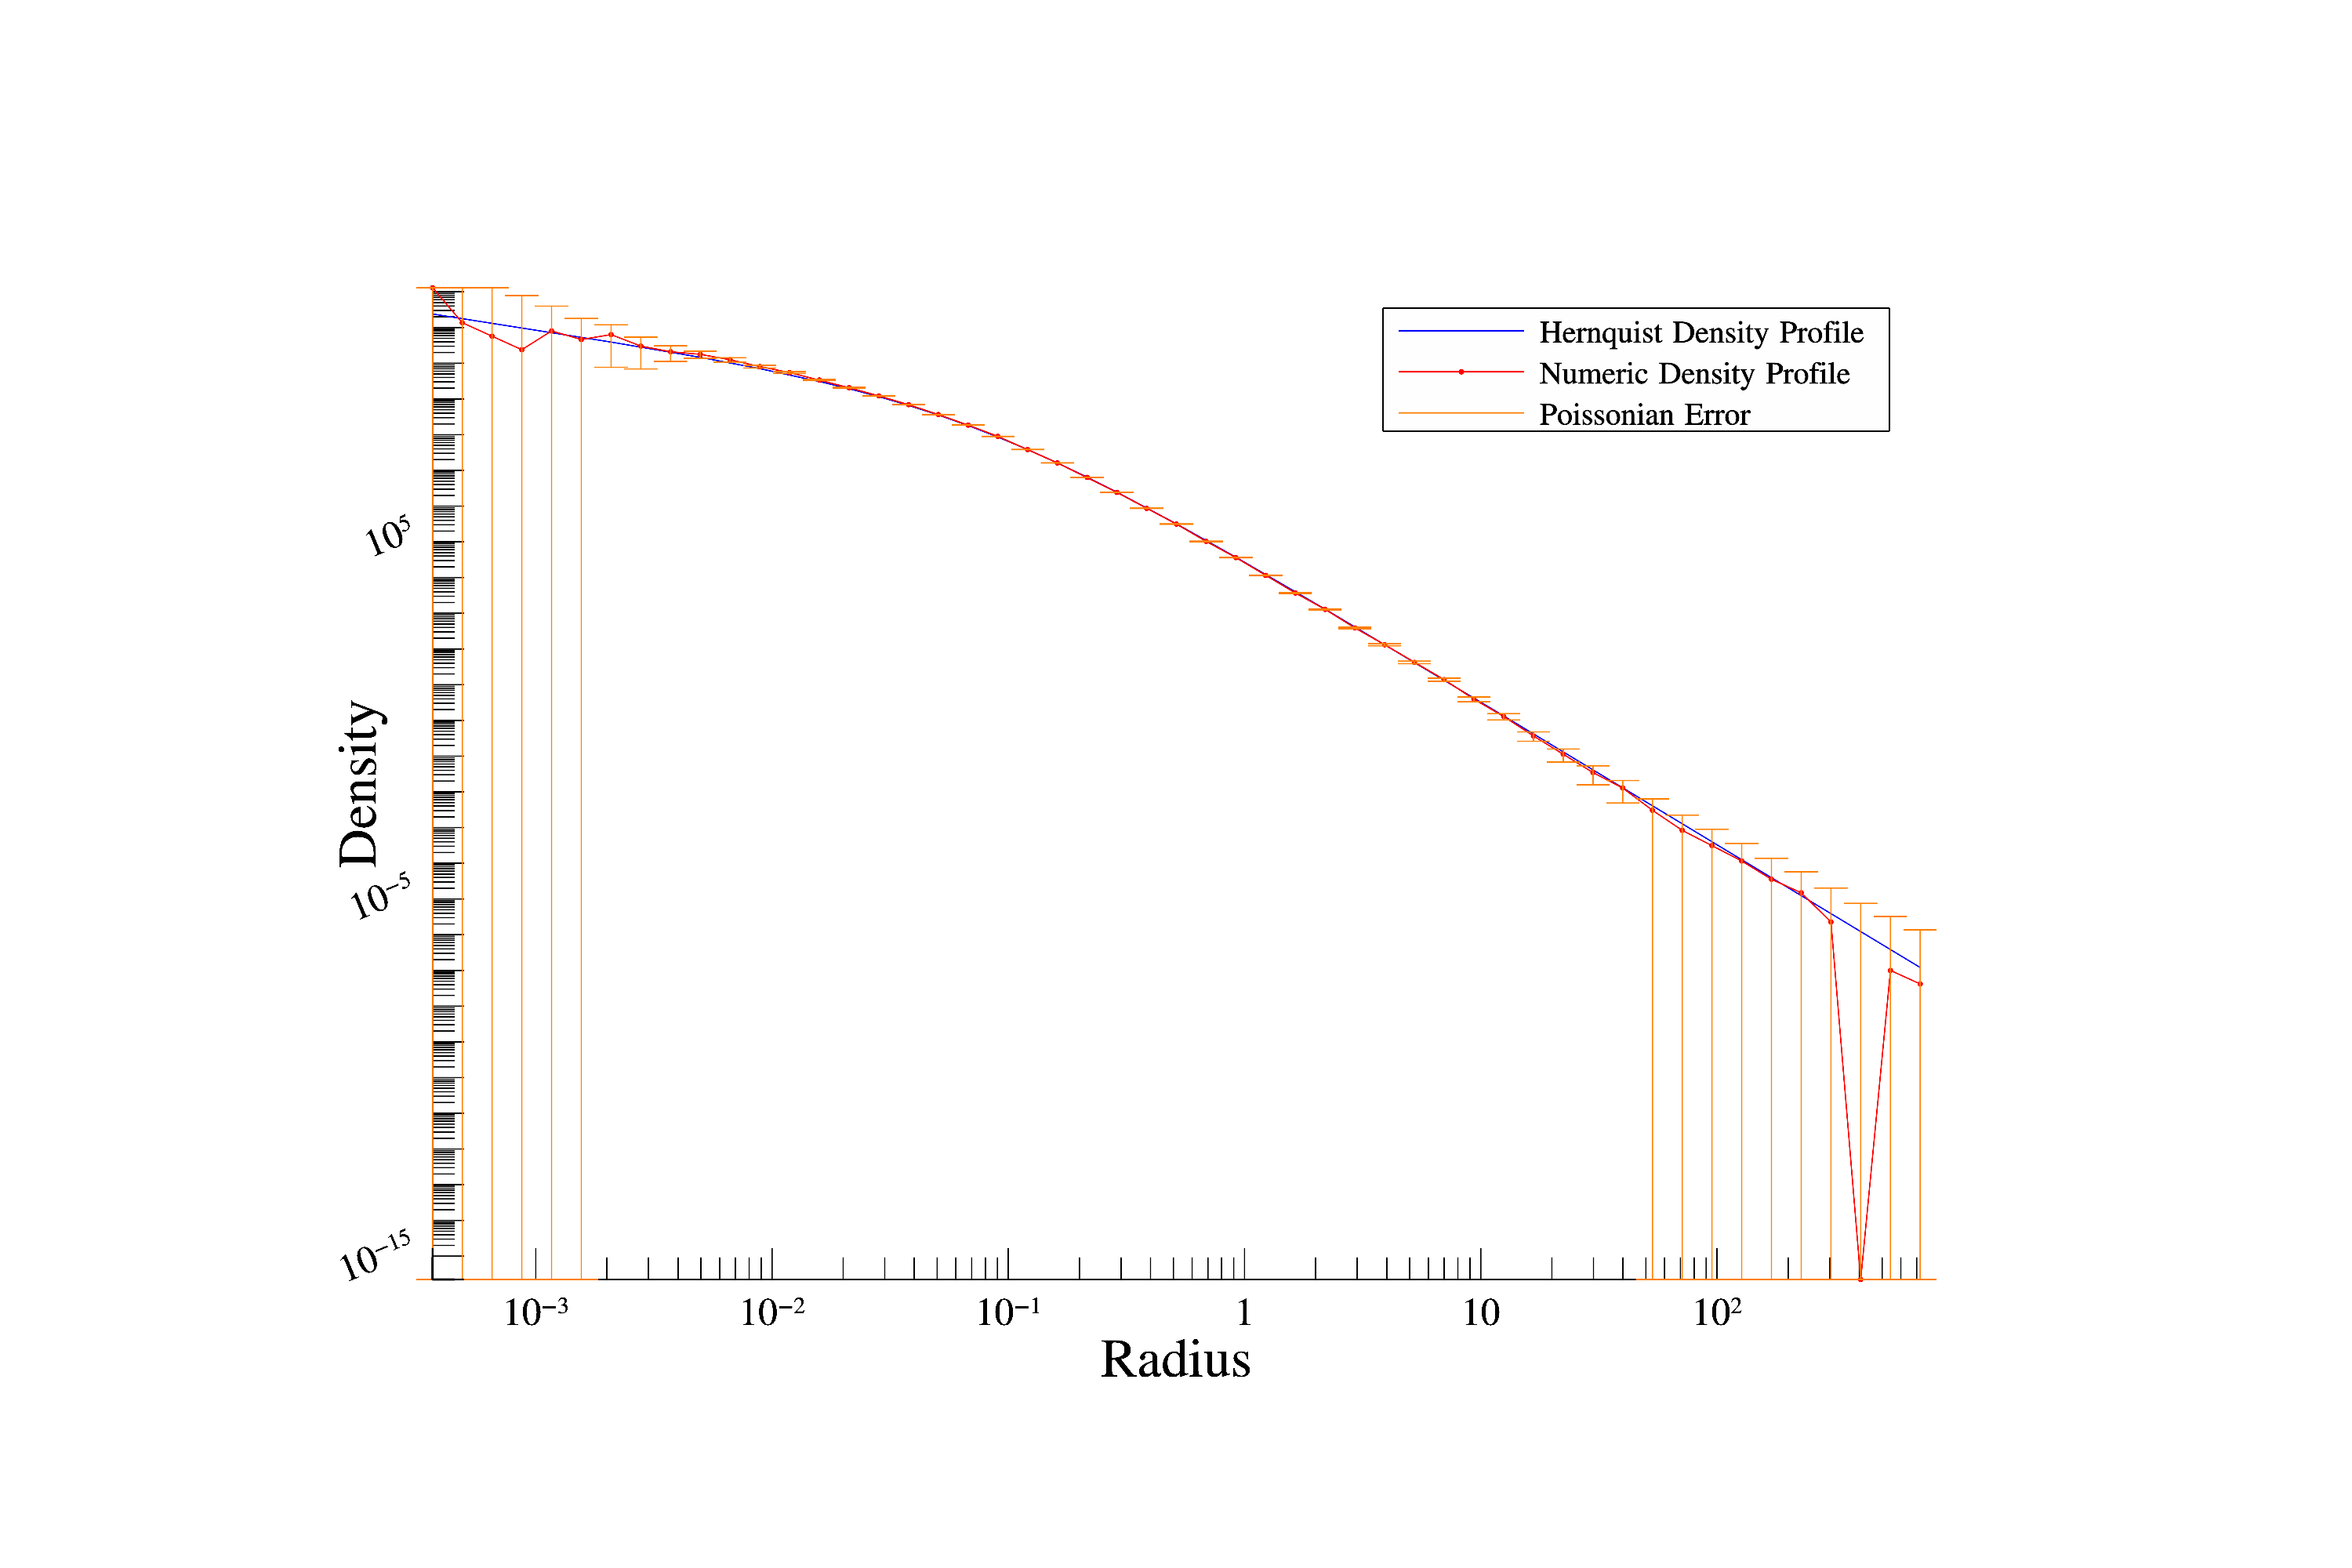
\includegraphics[width=1\textwidth]{figures/plots/hernquist.png}
\end{frame}

\subsection{Step 2: Direct Force Calculation}
\begin{frame}{Step 2: Analytic Force Reference}

	Assuming a Spherical System \cite{2008gady}, substituting $M(r)$ from Eq.
	(\ref{eq:cumulative-mass-distribution}) and reducing:
	\begin{equation}
		F(r) = - \frac{GM(r)}{r^2} \Rightarrow F(r) = - \frac{M}{(r+a)^2}
	\end{equation}

	{\footnotesize Where:
	\begin{itemize}
		\item $M$ - Total Mass of System
		\item $r$ - Radius of shell
		\item $a$ - Scale length of System
	\end{itemize}}
\end{frame}

\begin{frame}{Step 2: Direct Force Calculation}
	Keeping in mind $G=1$:
	\begin{equation}
		F_i=-G m_i \sum_{j=1}^N \frac{m_j}{\left[\left(\vb{r}_i-\vb{r}_j\right)^2+\varepsilon^2\right]^{3 /
				2}}\left(\vb{r}_i-\vb{r}_j\right)
	\end{equation}

	Softening equation (2.227) from \textit{Galactic Dynamics}:
	\begin{equation}
		\epsilon=-\frac{r_{max}^2+\frac{3}{2} a^2}{\left(r_{max}^2+a^2\right)^{3 / 2}}
	\end{equation}
	or, as suggested, substituting $a$ from above with:
	\begin{equation}
		d=\left[\frac{(4 \pi / 3) R_{hm}^3}{N}\right]^{1 / 3}
	\end{equation}

	{\footnotesize Where:
	\begin{itemize}
		\item $i$ - Particle under consideration
		\item $\epsilon$ - Softening: accurate at $\approx 10^{-5}$
		\item $r_{max}$ - Maximum radius
		\item $d$ - Mean inter-particle separation
		\item $a$ - Scale length
		\item $G=1$
	\end{itemize}
	}
\end{frame}

\begin{frame}{Step 2: Direct Force Calculation}
	Vectors converted to scalars by \textbf{normalizing} the Force vector and \textbf{projecting} it on the center
	for numeric approximation and analytic comparison:
	\begin{equation}
		F_{avg}^b = \frac{1}{N_{Bin}} \sum^{N_{Bin}}_{i=0} \frac{\vb{r}_i\cdot \vb{F}_i}{|\vb{r}_i|}
	\end{equation}

	{\footnotesize Where:
	\begin{itemize}
		\item $N_{Bin}$ - Number of particles in a bin or shell
		\item $\vb{r}_i$ - Position vector of particle i
		\item $\vb{F}_i$ - Force Vector of particle i
		\item $F_{avg}^b$ - Average force on bin $b$
	\end{itemize}
	}
\end{frame}

\begin{frame}{Softening /= 1, with $a$}
	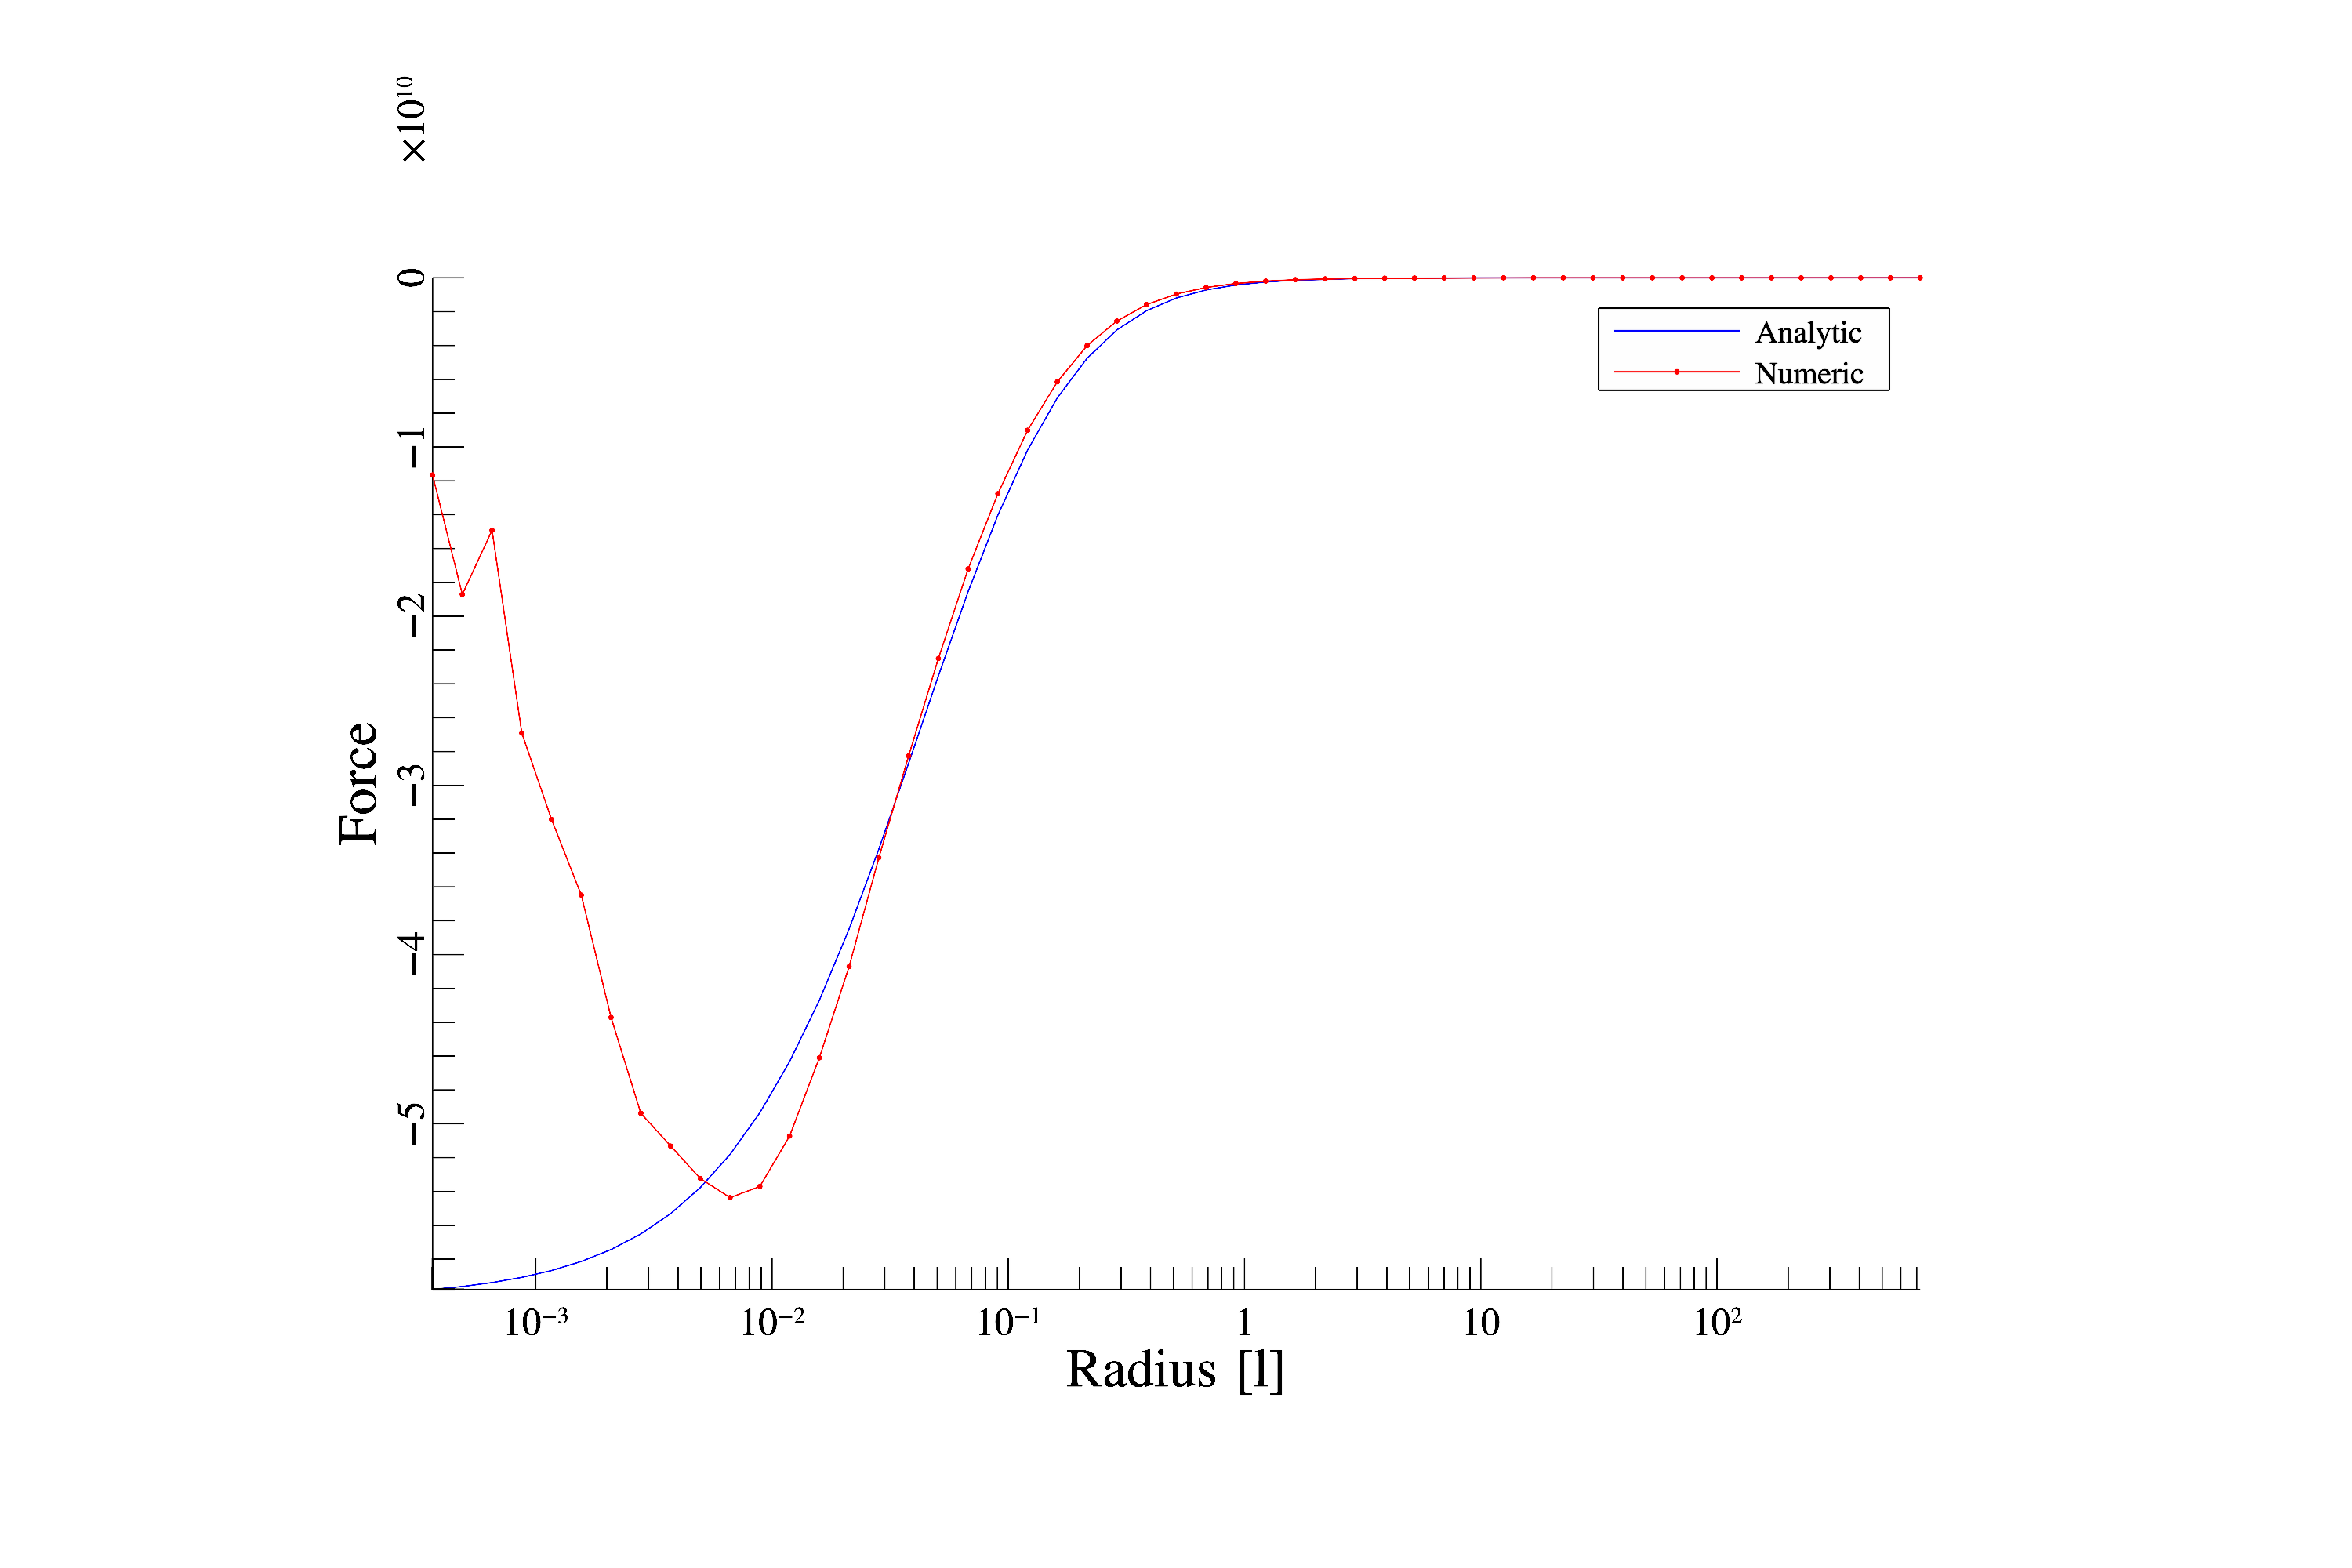
\includegraphics[width=0.95\textwidth]{figures/plots/forces_a_1.png}
\end{frame}

\begin{frame}{Softening /= 8, with $a$}
	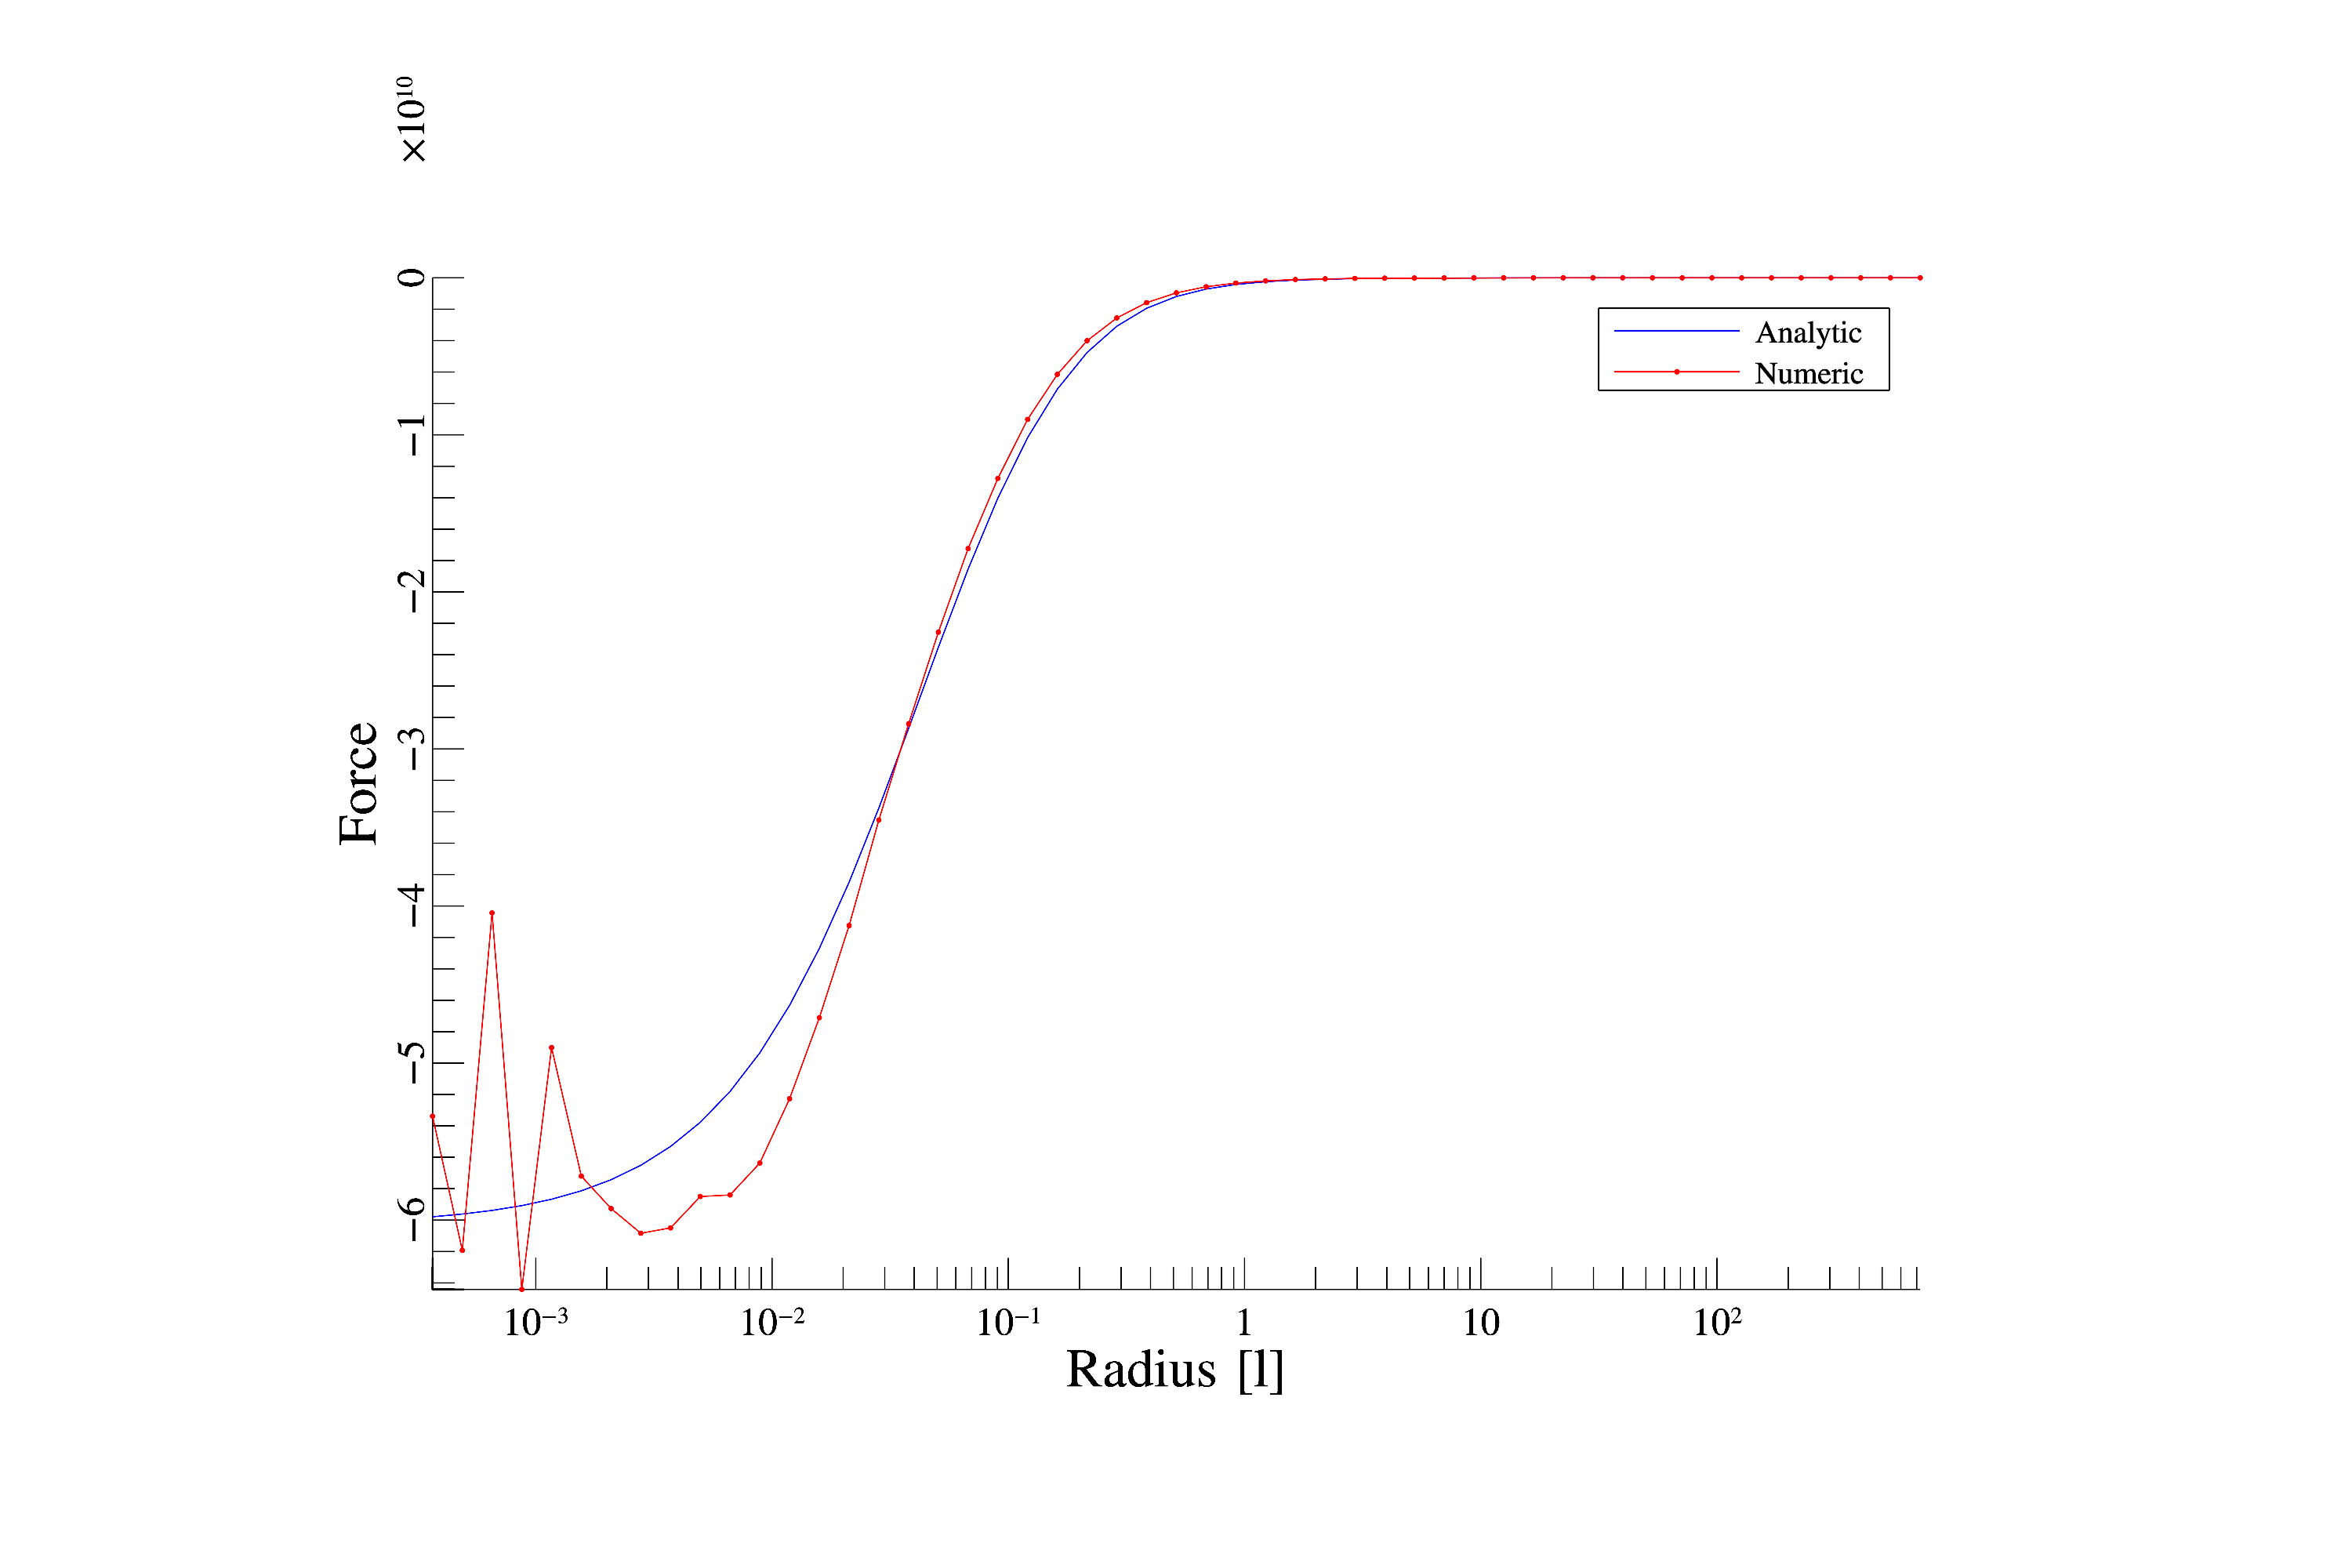
\includegraphics[width=0.95\textwidth]{figures/plots/forces_a_8.png}
\end{frame}

\begin{frame}{Softening /= 16, with $a$}
	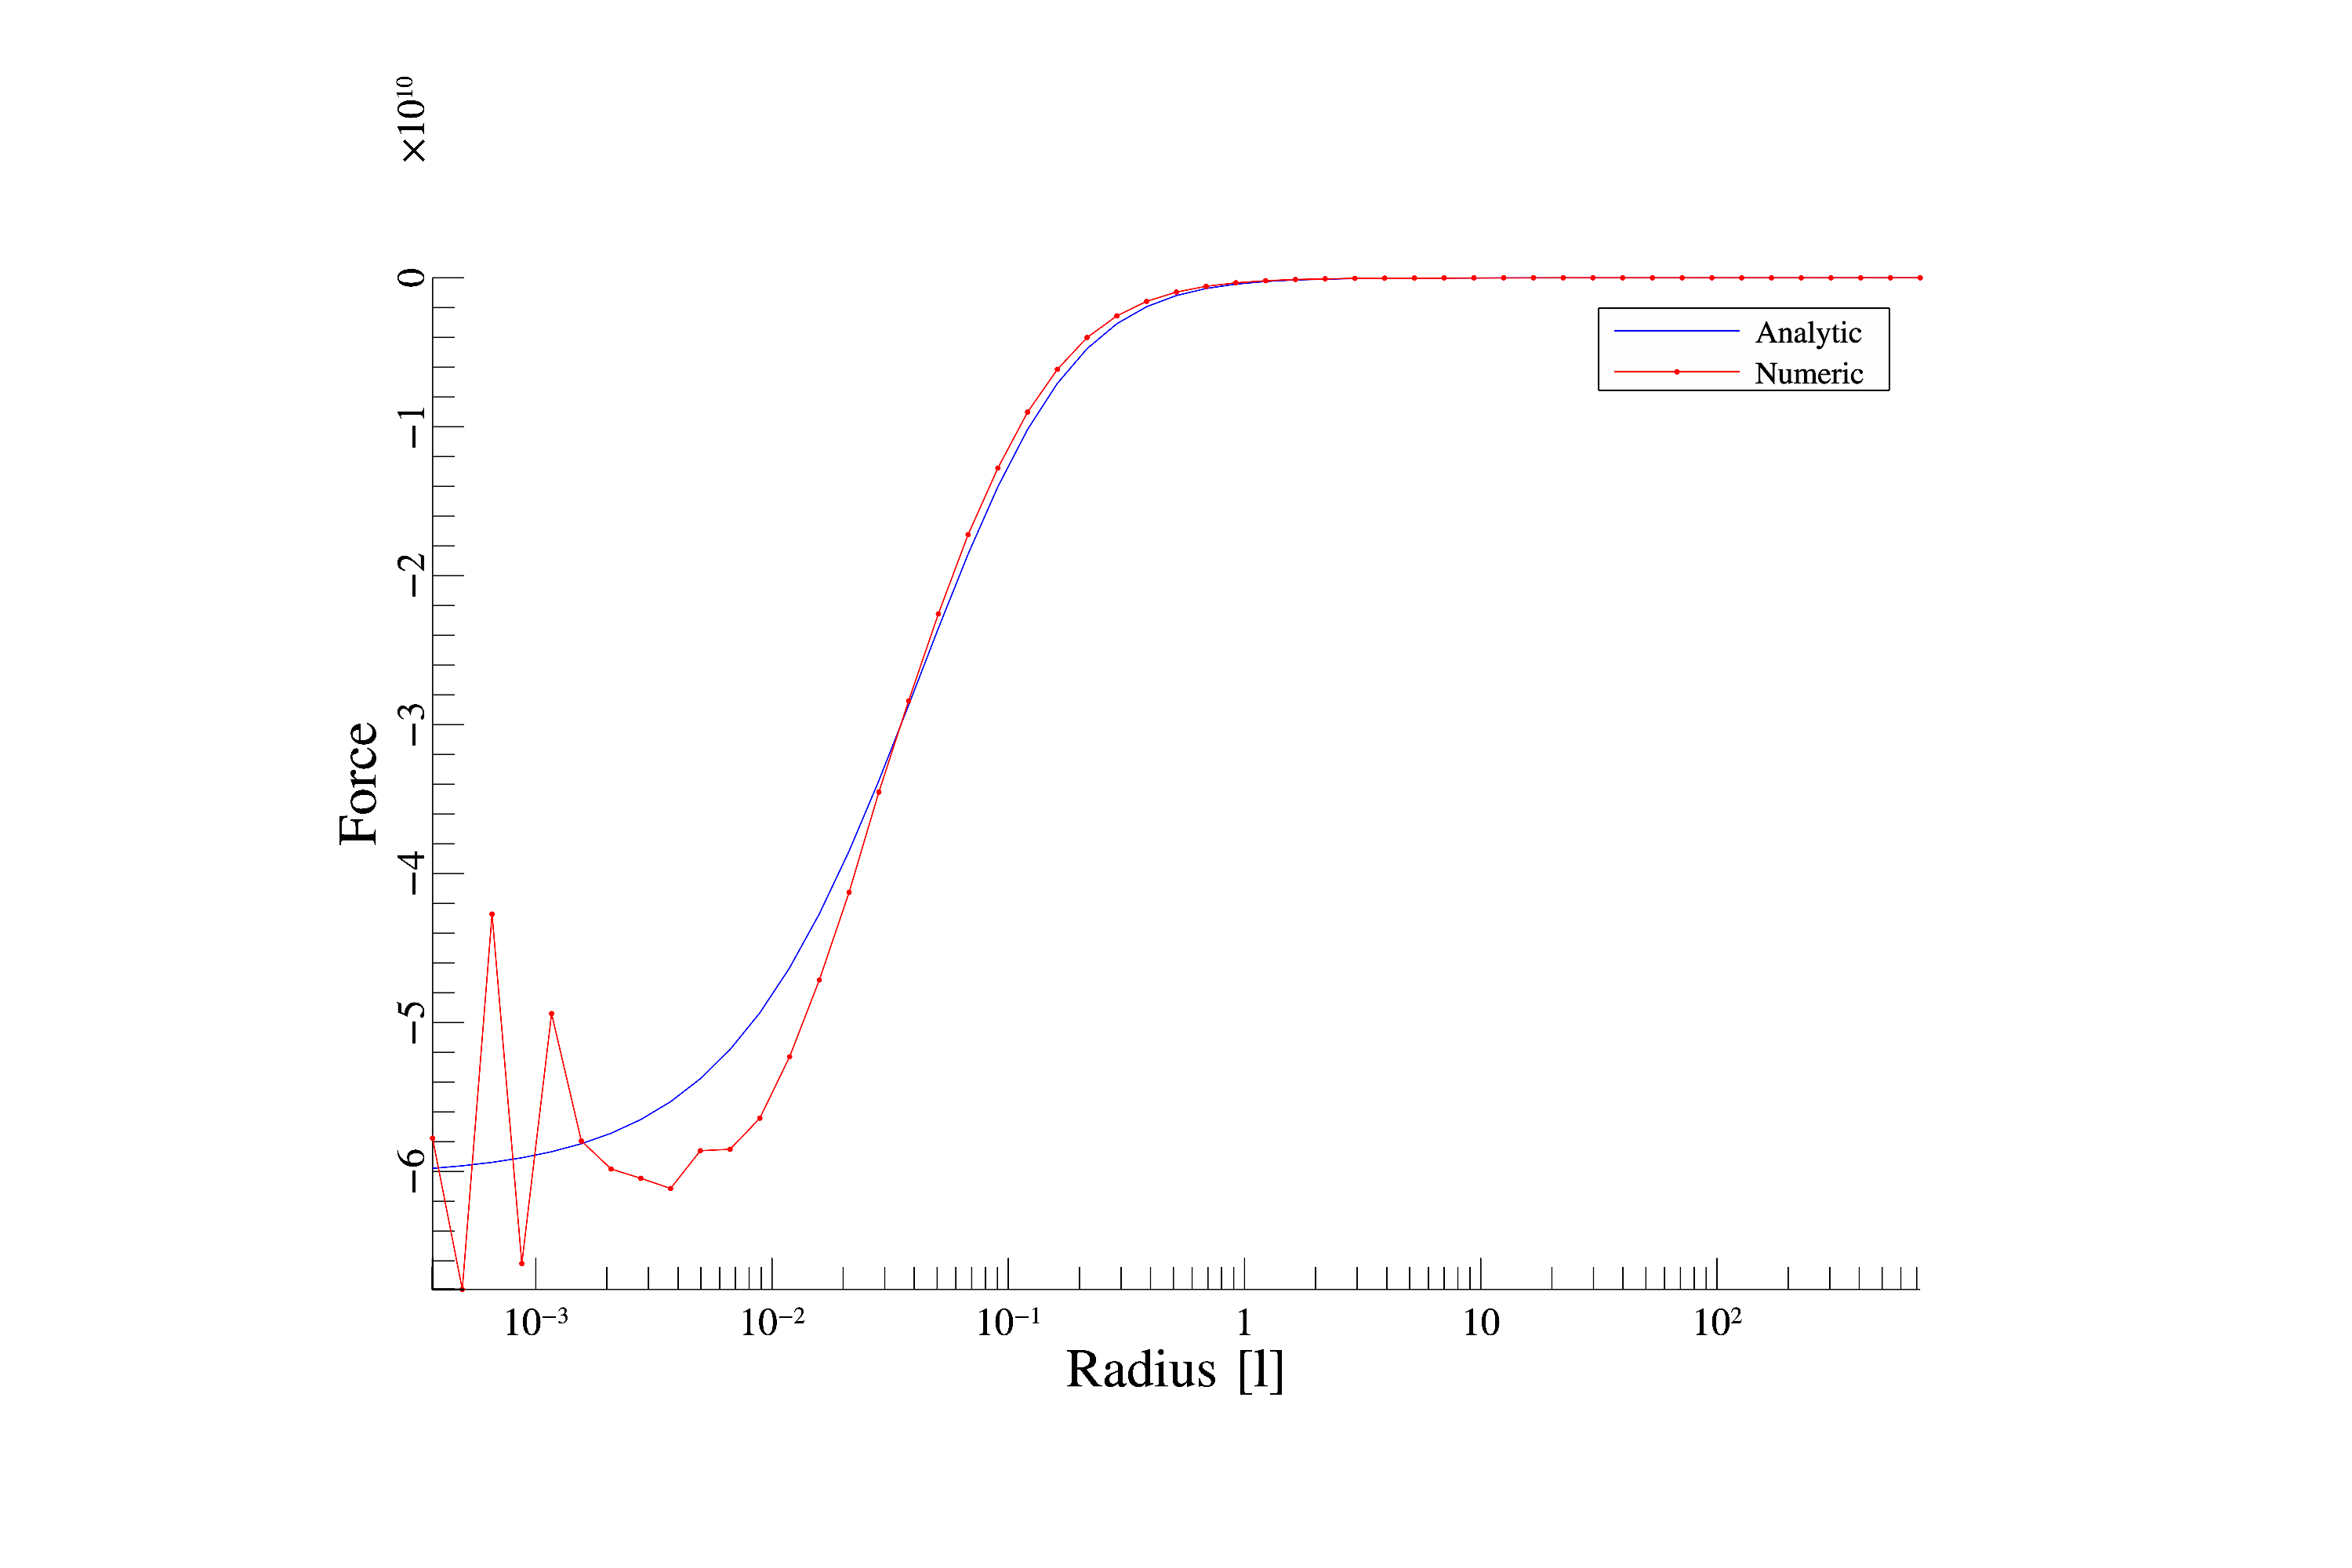
\includegraphics[width=0.95\textwidth]{figures/plots/forces_a_16.png}
\end{frame}

\begin{frame}{Softening /= 32, with $a$}
	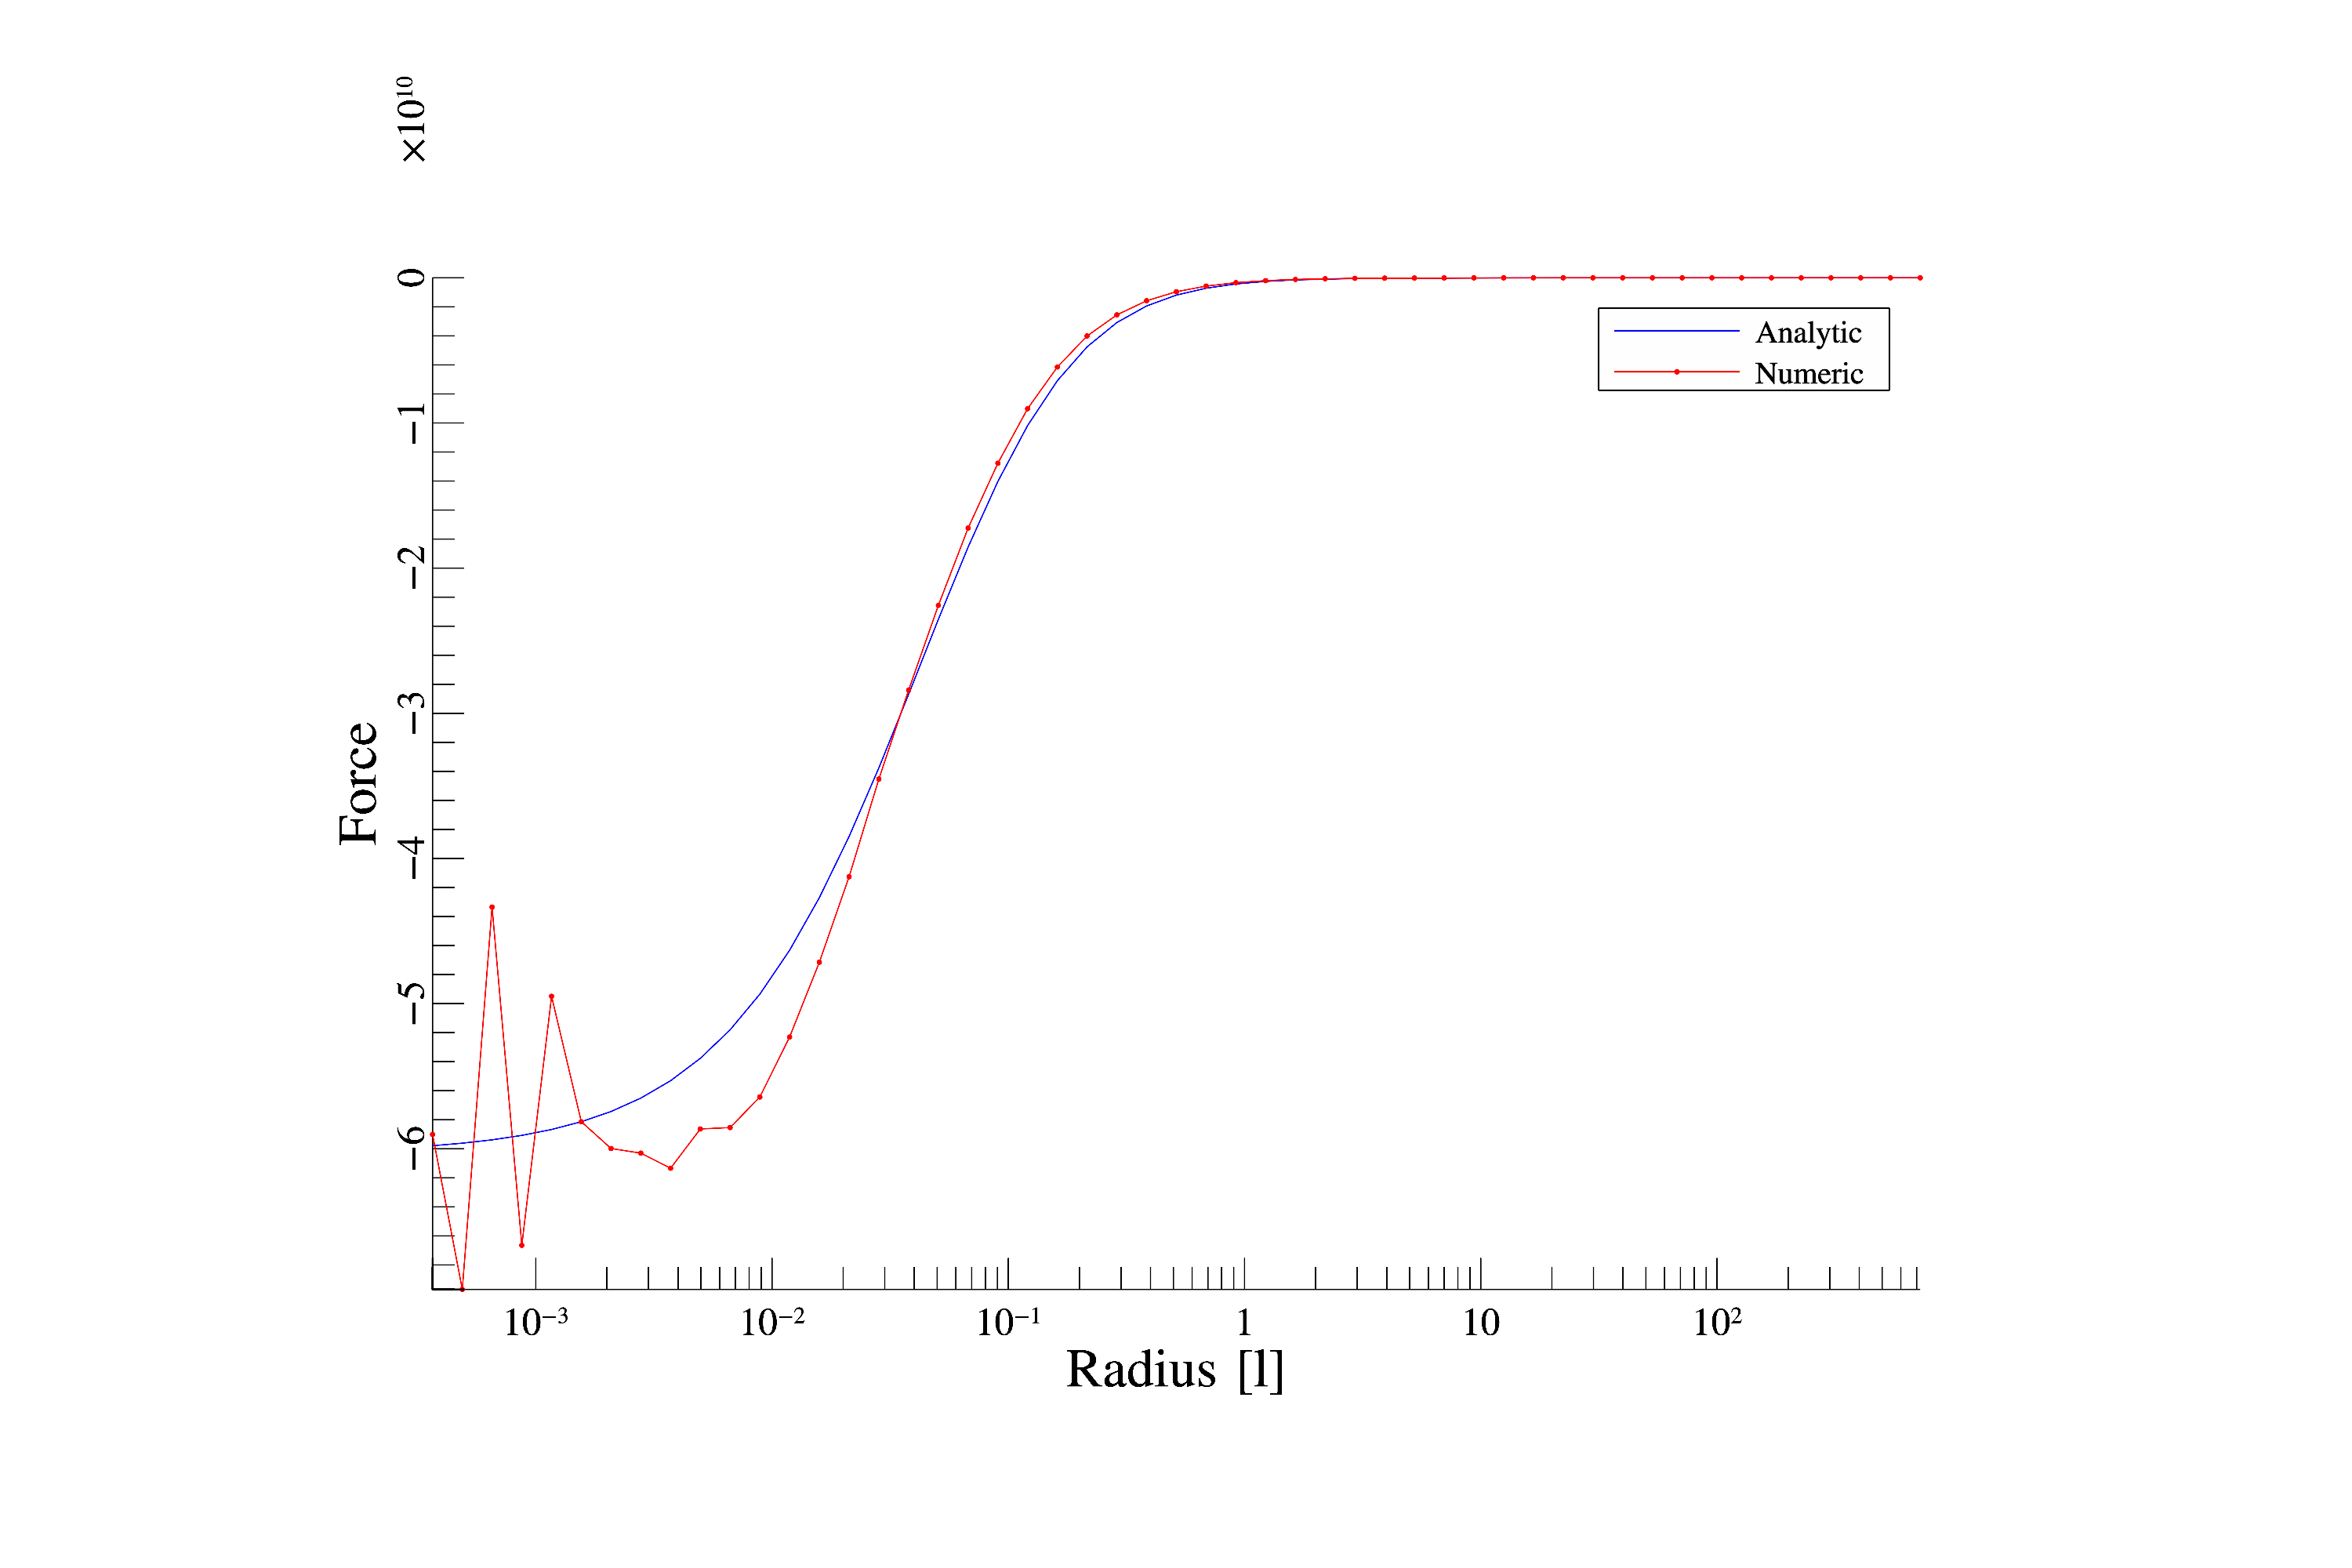
\includegraphics[width=0.95\textwidth]{figures/plots/forces_a_32.png}
\end{frame}

\begin{frame}{Softening /= 64, with $a$}
	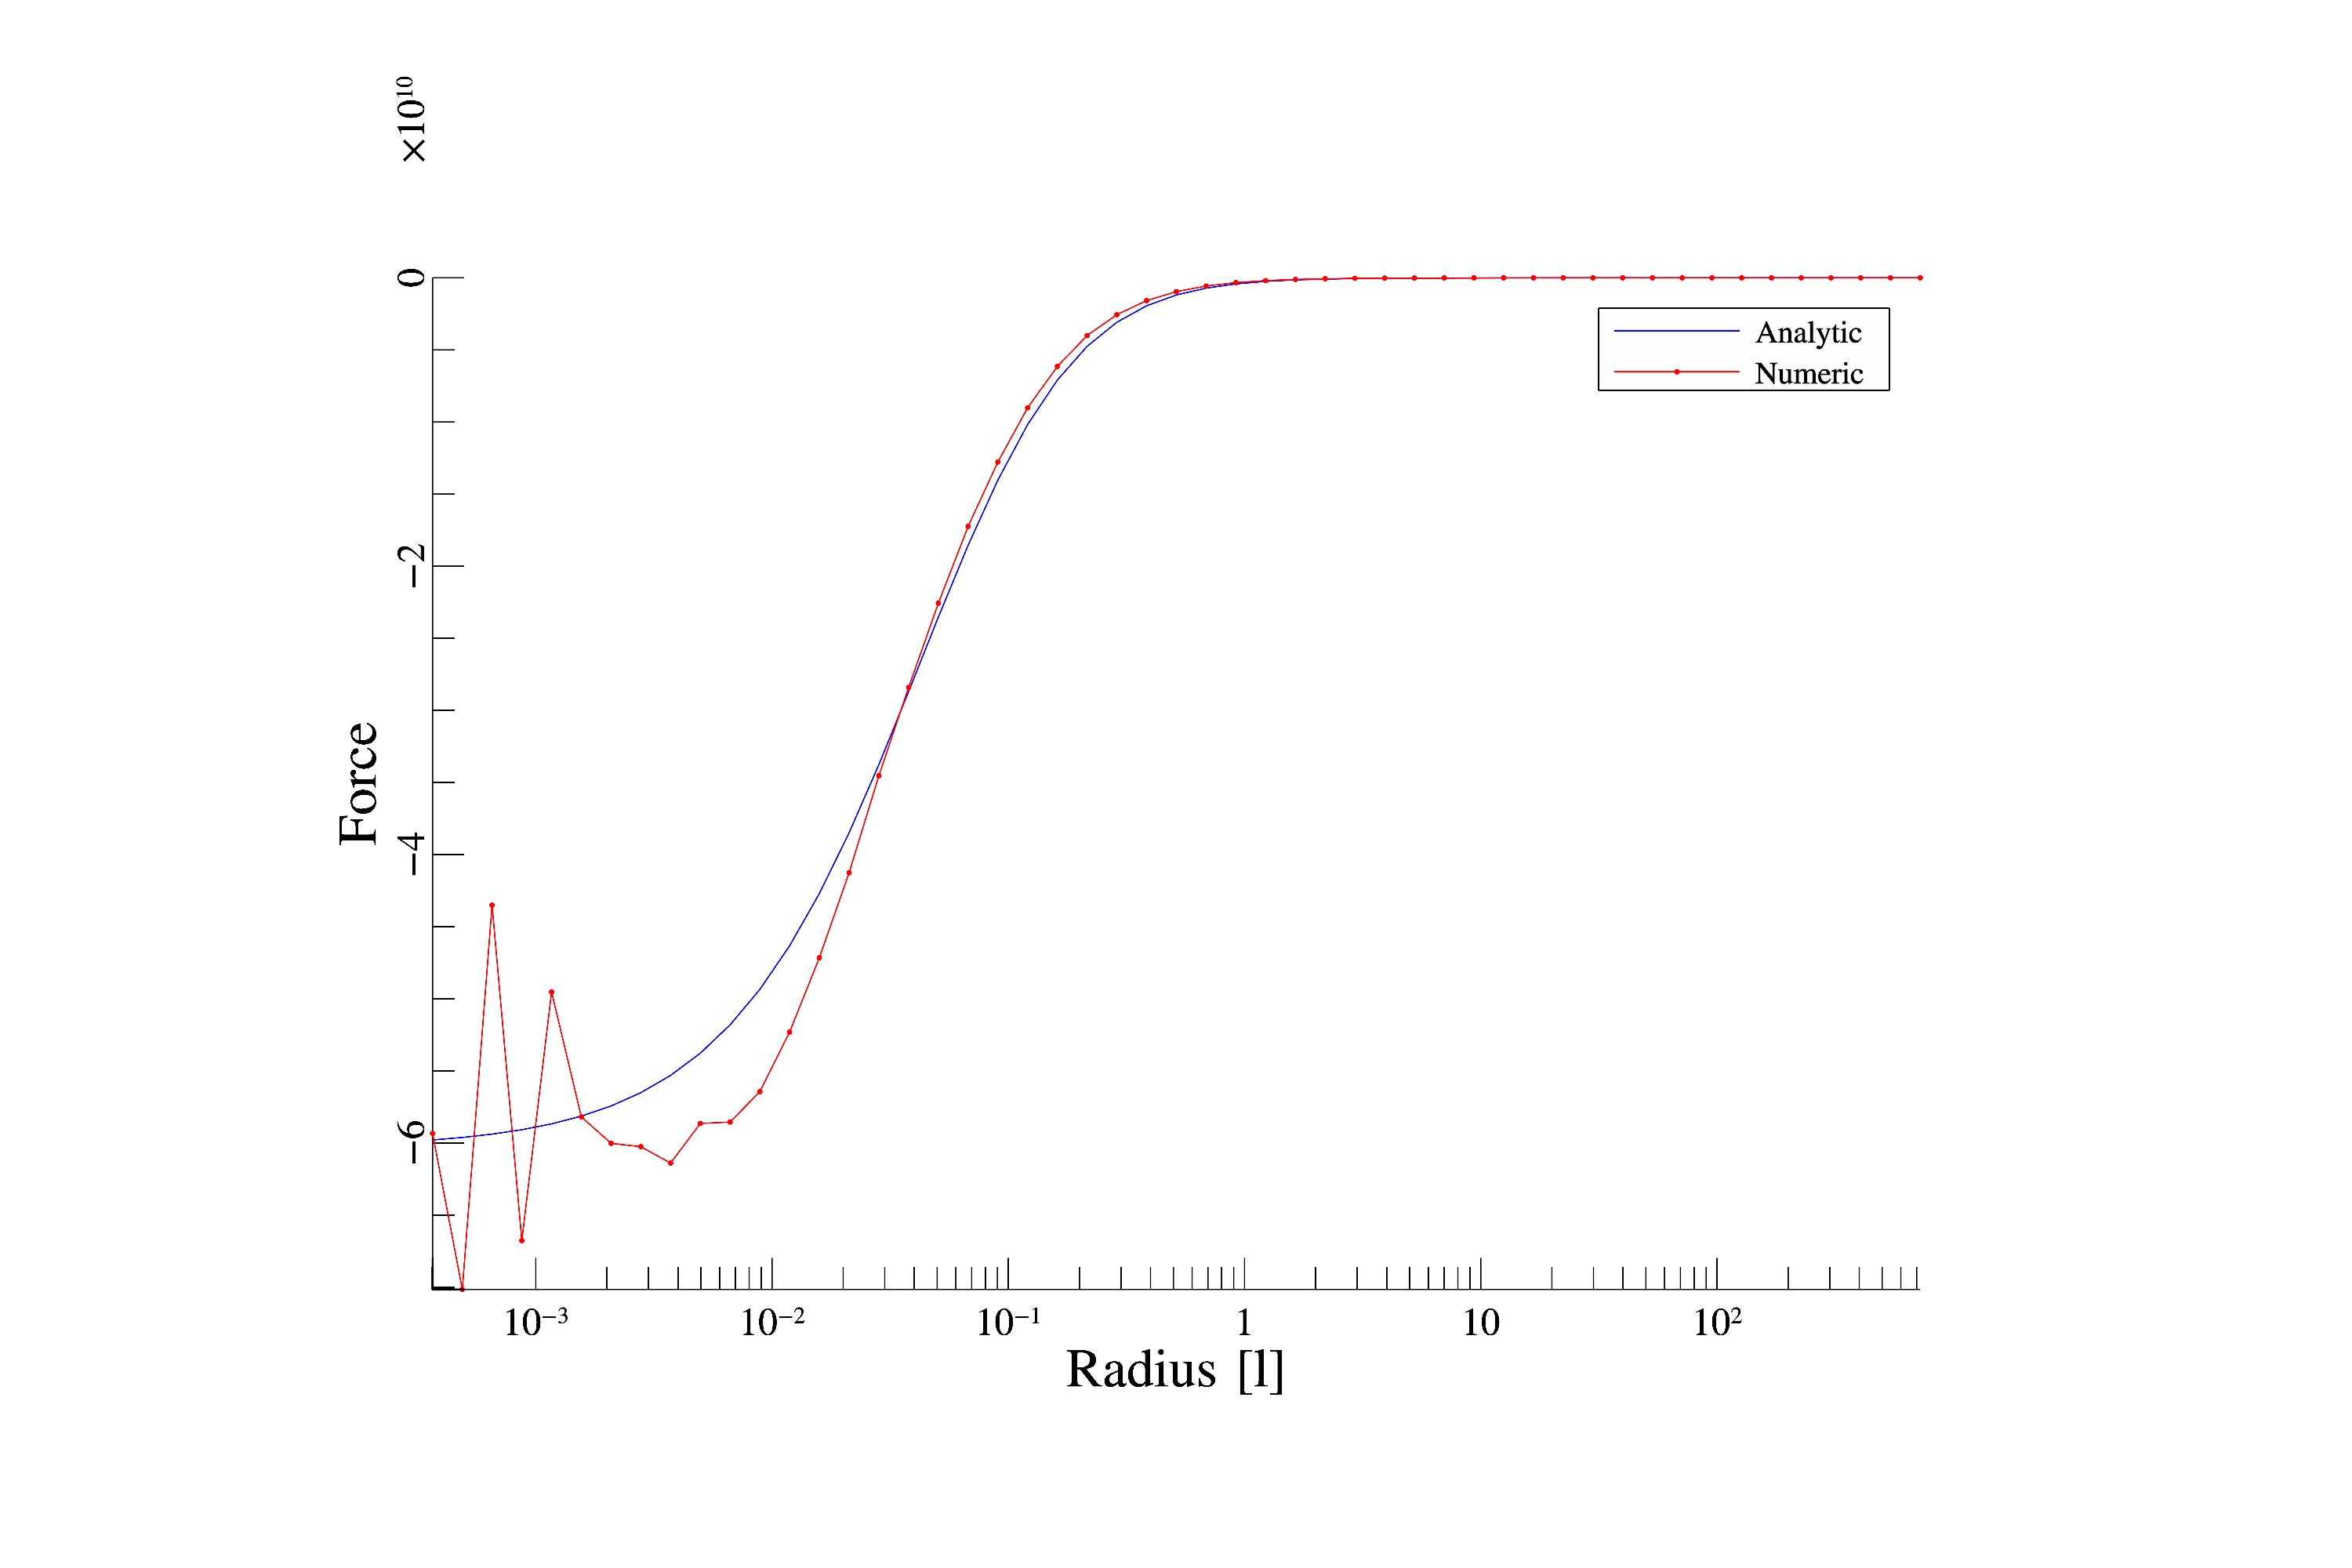
\includegraphics[width=0.95\textwidth]{figures/plots/forces_a_64.png}
\end{frame}

\begin{frame}{Softening /= 128, with $a$}
	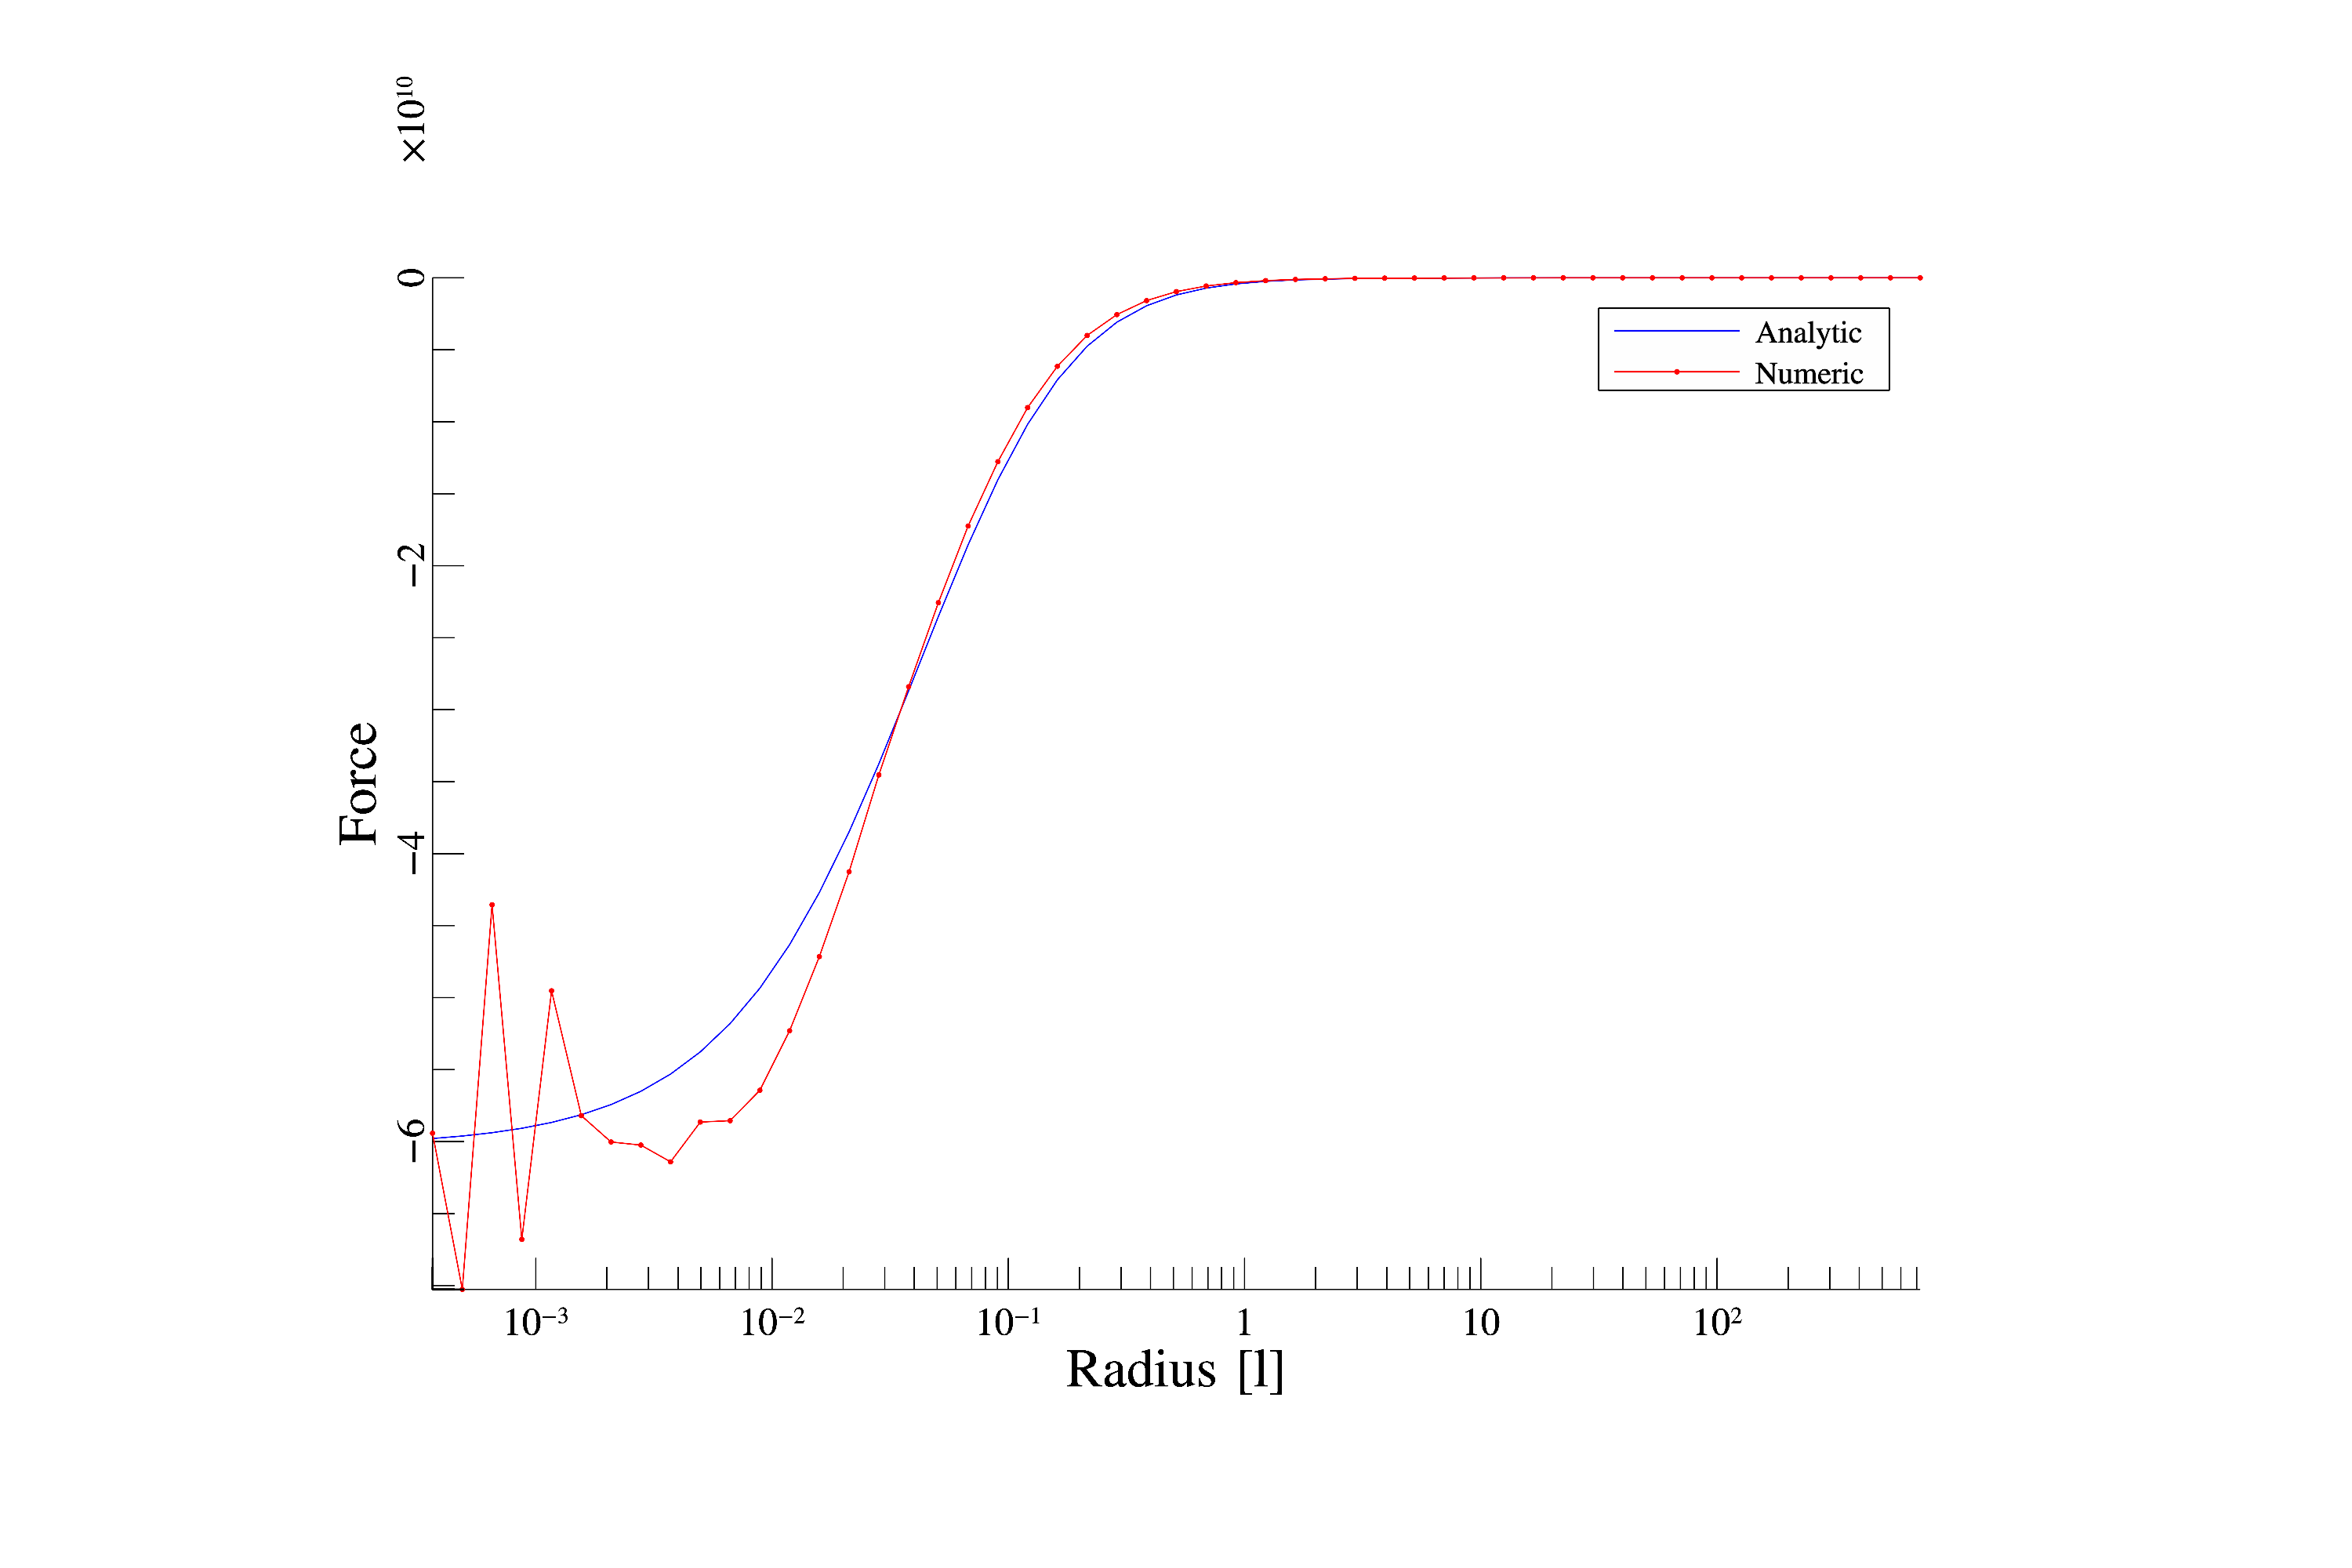
\includegraphics[width=0.95\textwidth]{figures/plots/forces_a_128.png}
\end{frame}

\begin{frame}{Softening /= 1, with $d$}
	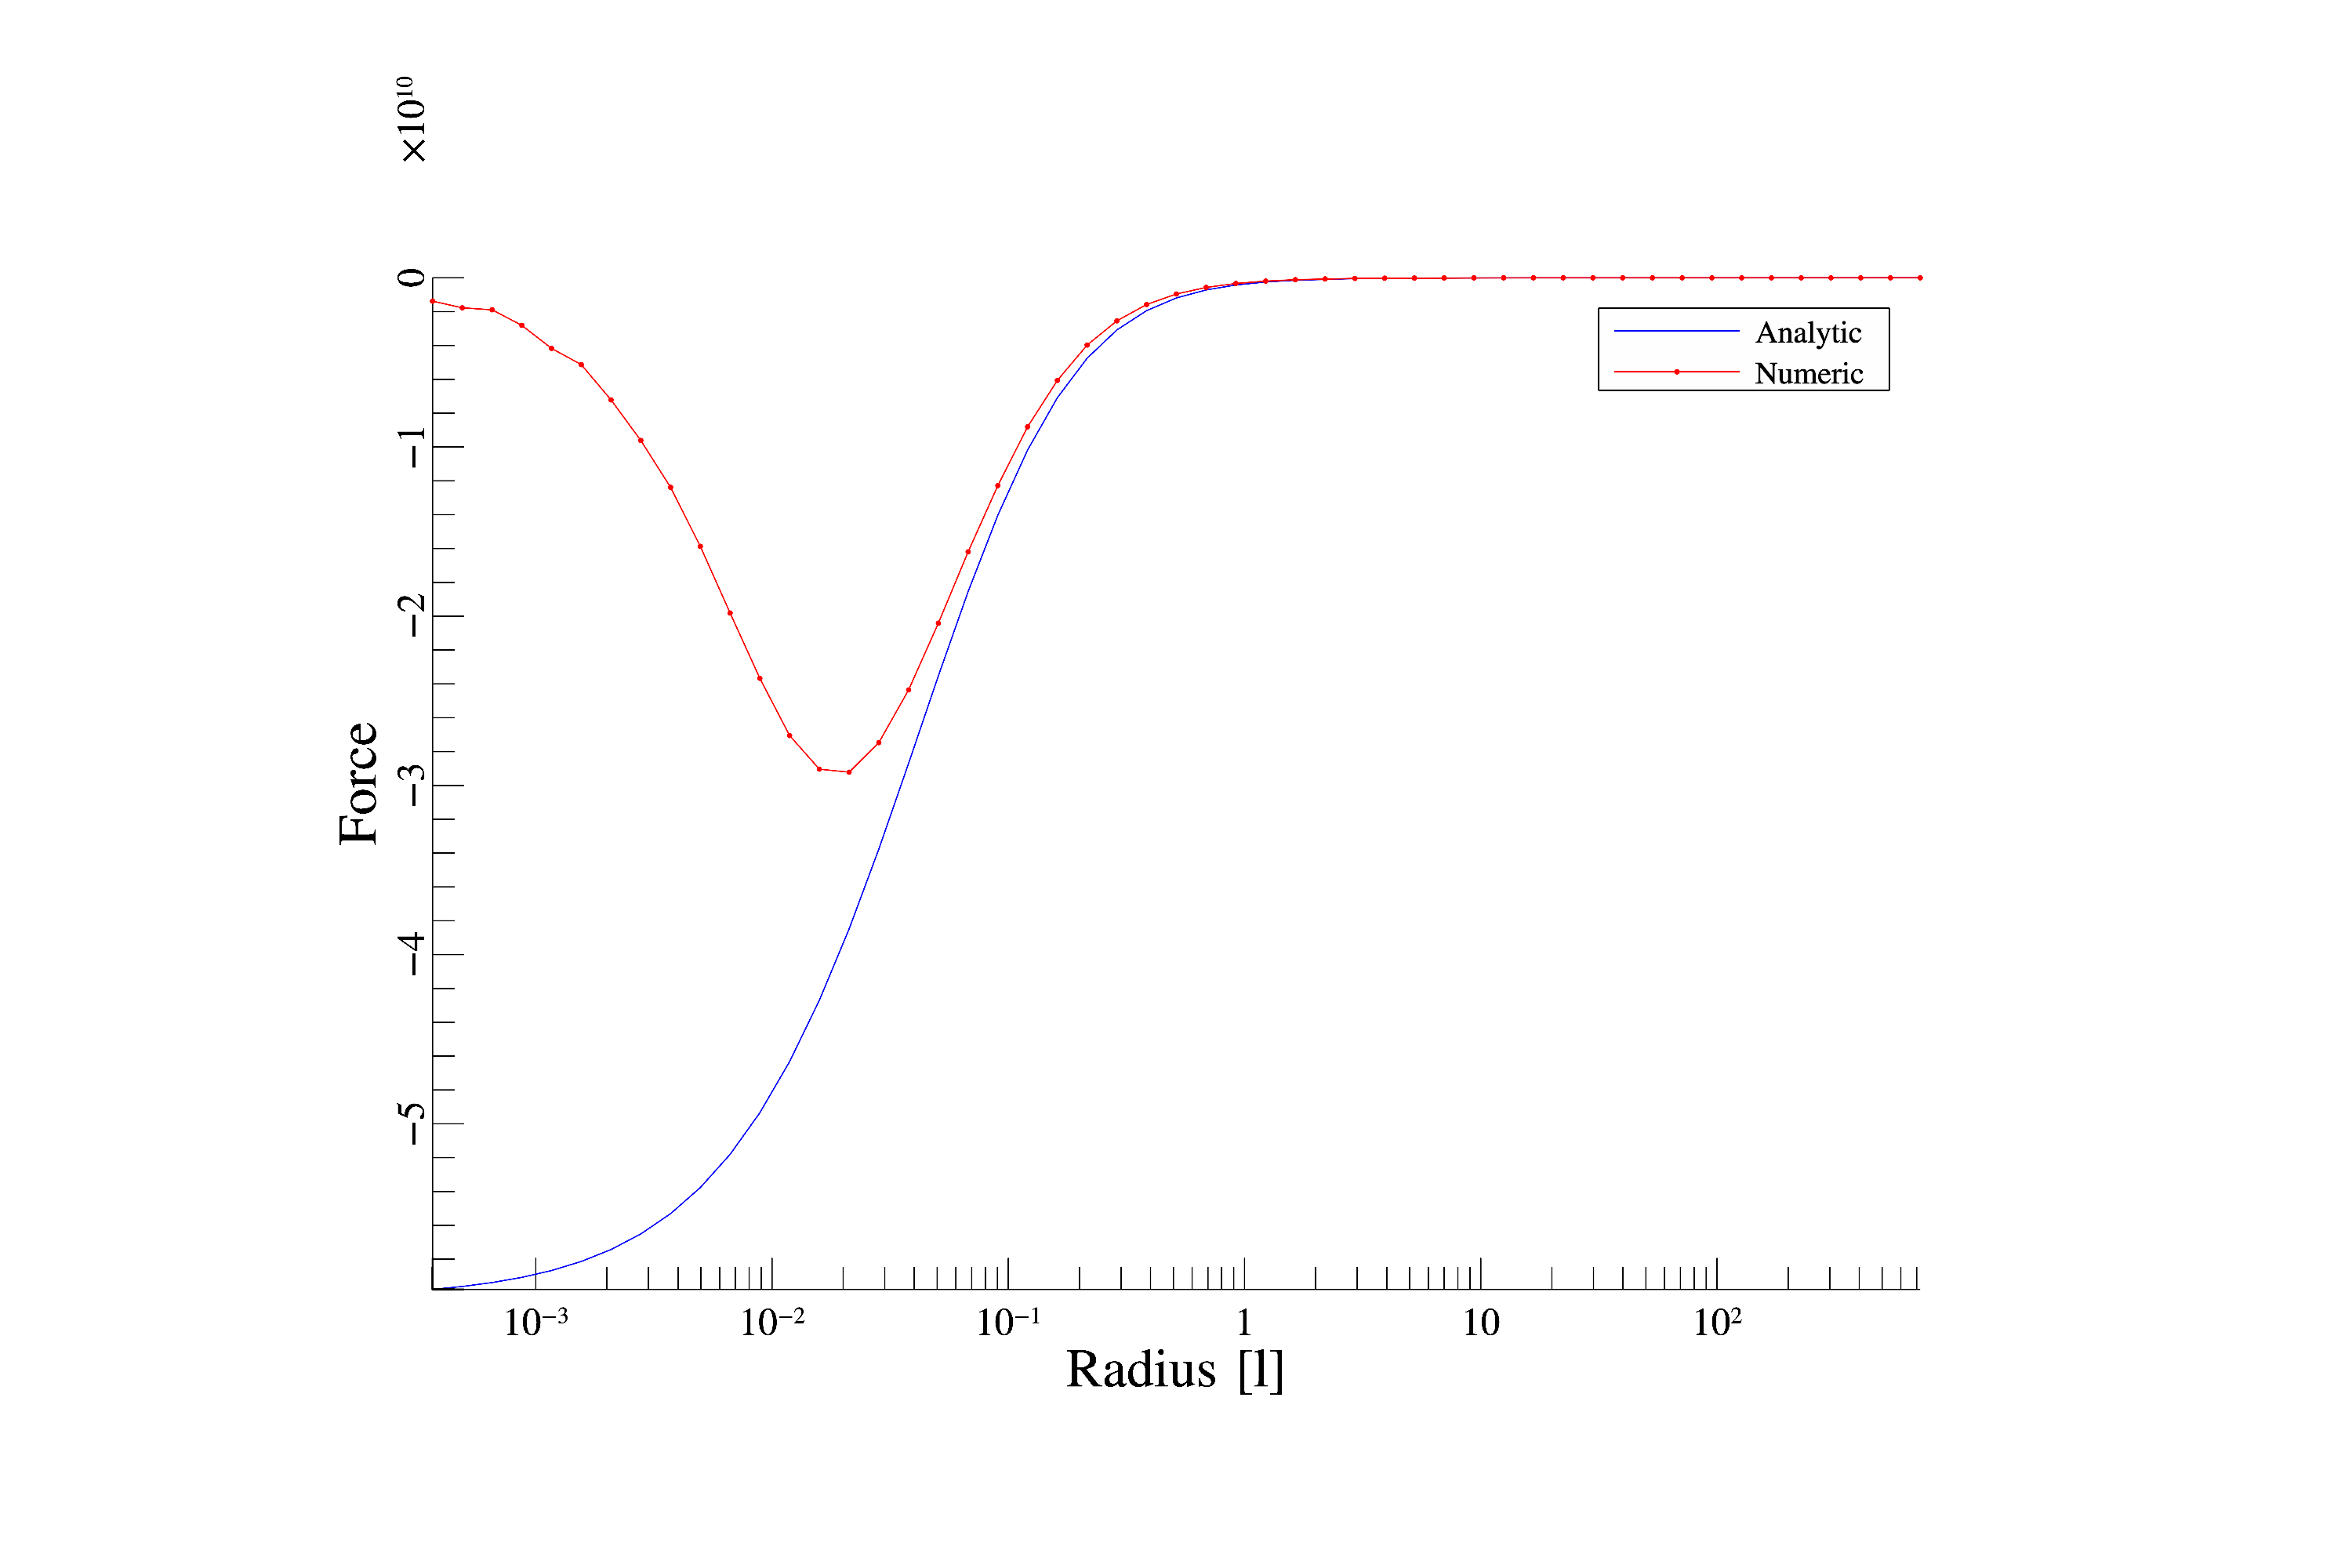
\includegraphics[width=0.95\textwidth]{figures/plots/forces_d_1.png}
\end{frame}

\begin{frame}{Softening /= 8, with $d$}
	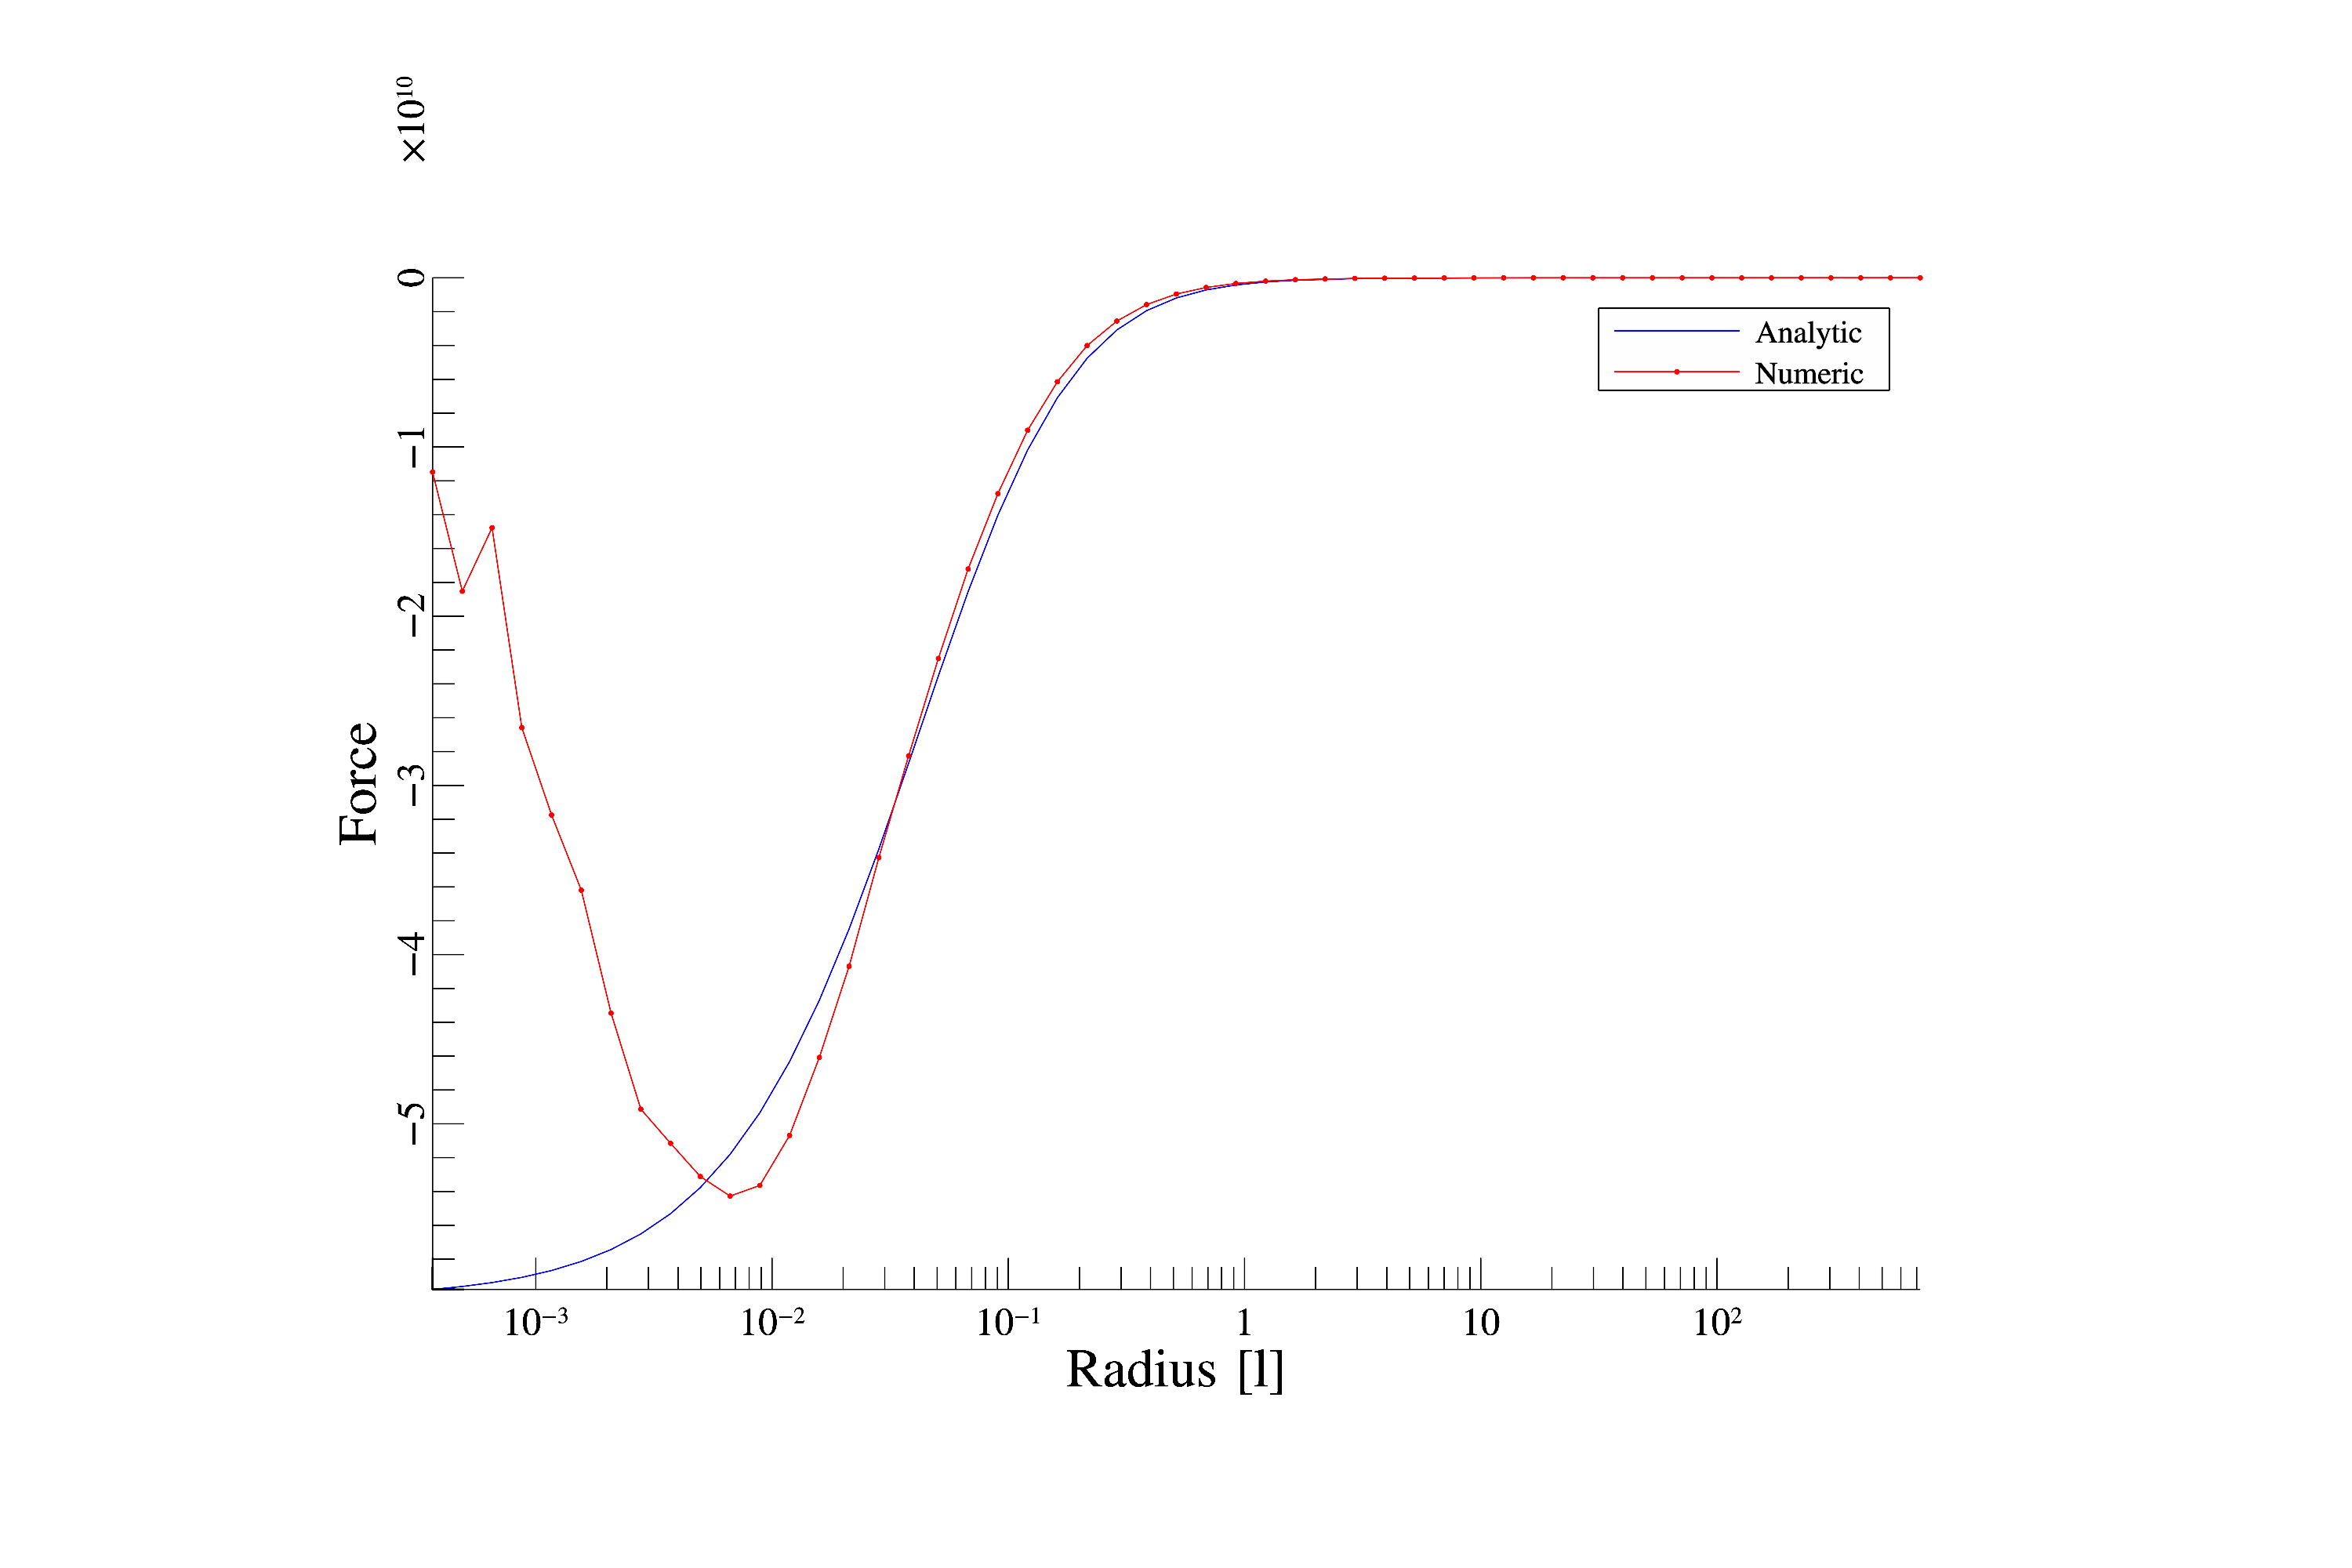
\includegraphics[width=0.95\textwidth]{figures/plots/forces_d_8.png}
\end{frame}

\begin{frame}{Softening /= 32, with $d$}
	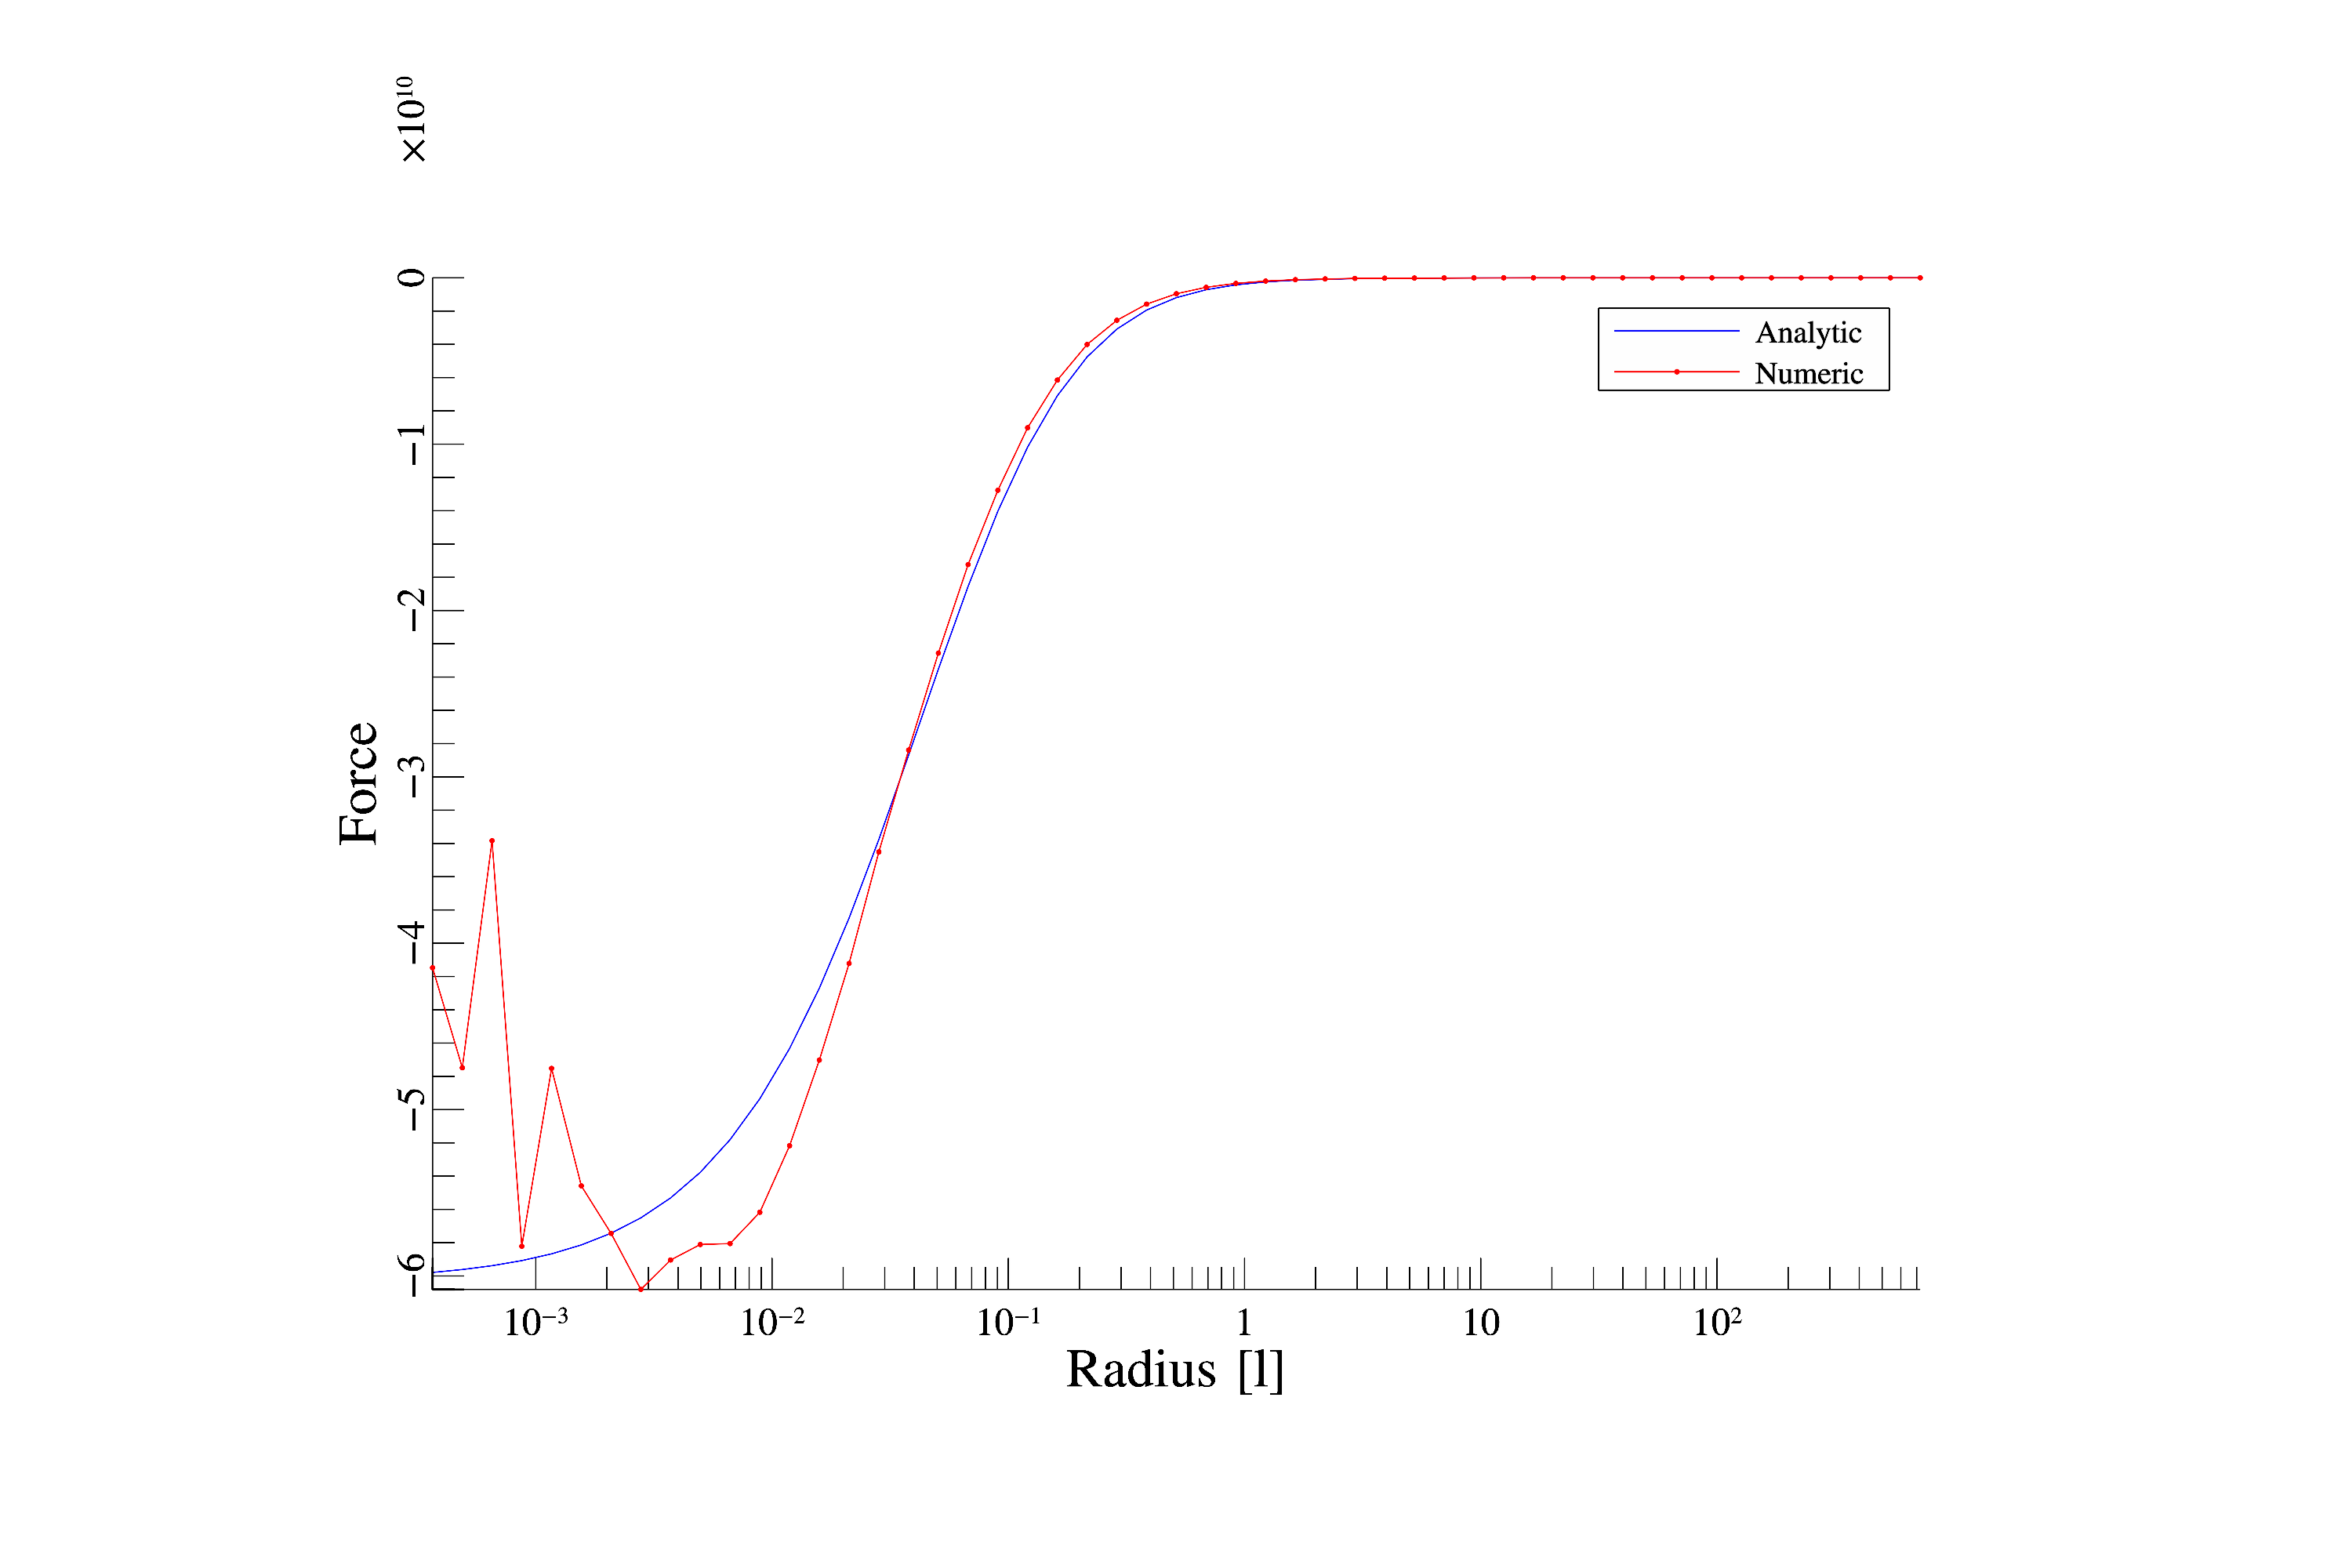
\includegraphics[width=0.95\textwidth]{figures/plots/forces_d_32.png}
\end{frame}

\begin{frame}{Softening /= 64, with $d$}
	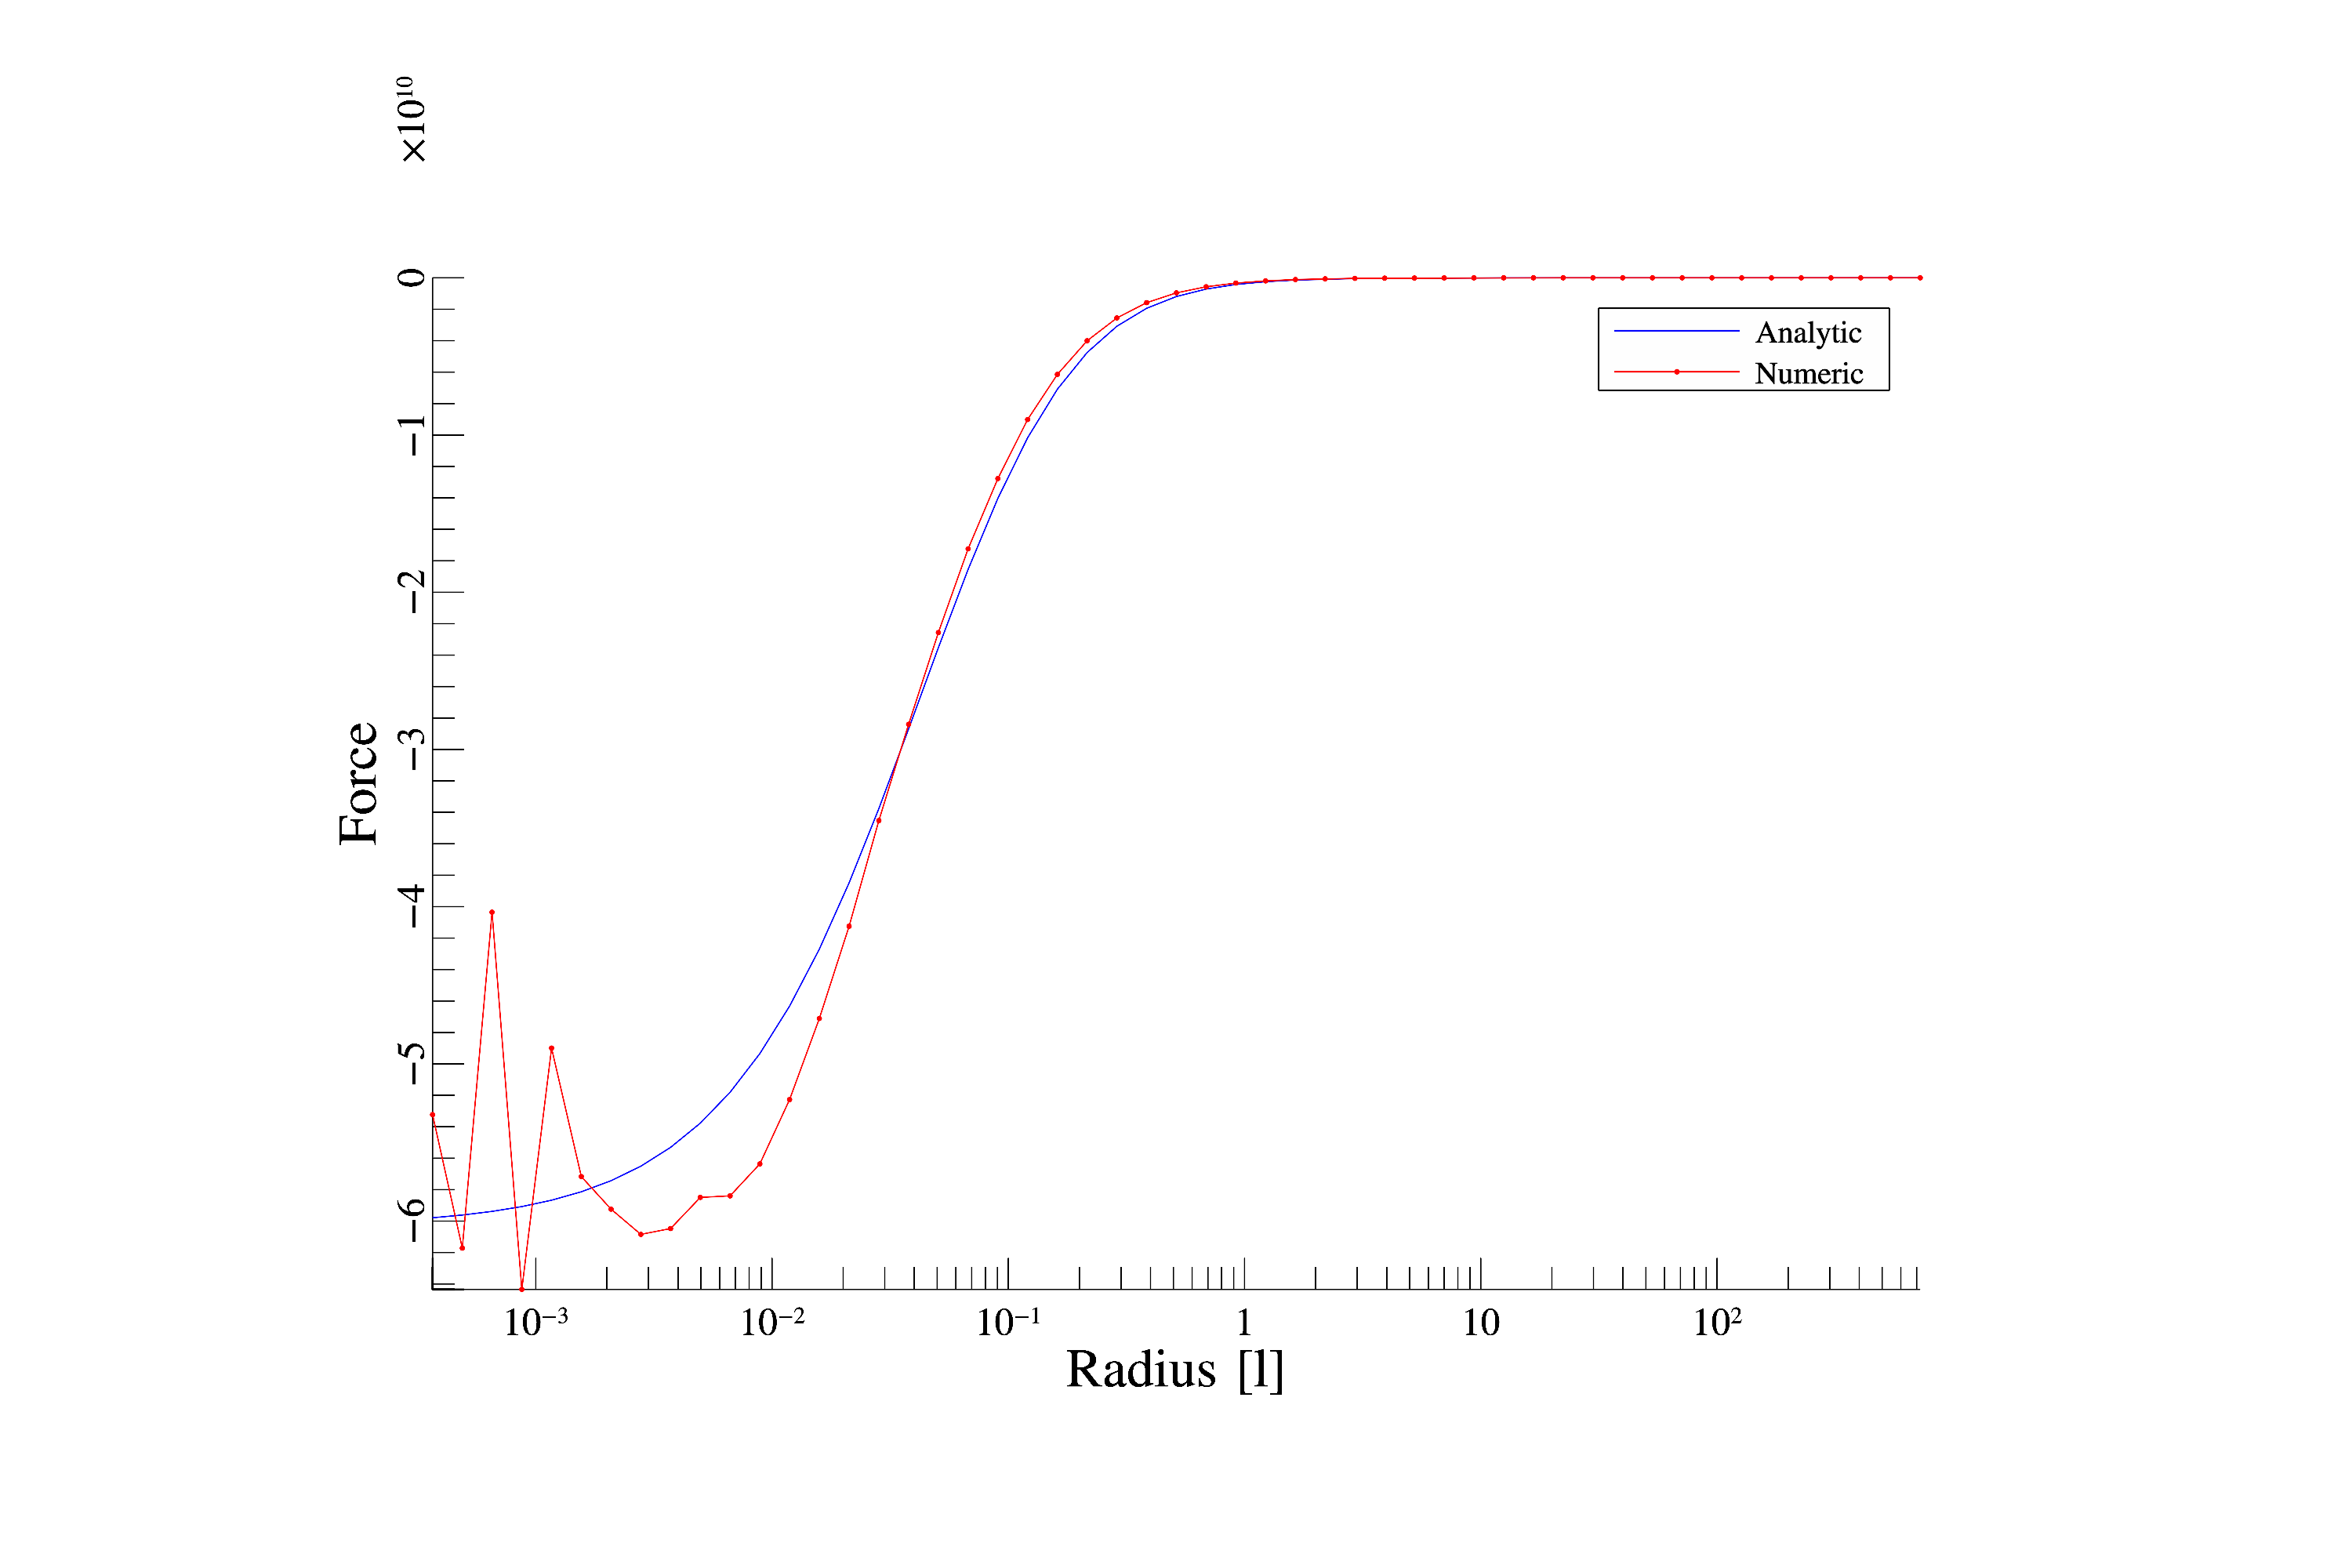
\includegraphics[width=0.95\textwidth]{figures/plots/forces_d_64.png}
\end{frame}

\begin{frame}{Softening /= 128, with $d$}
	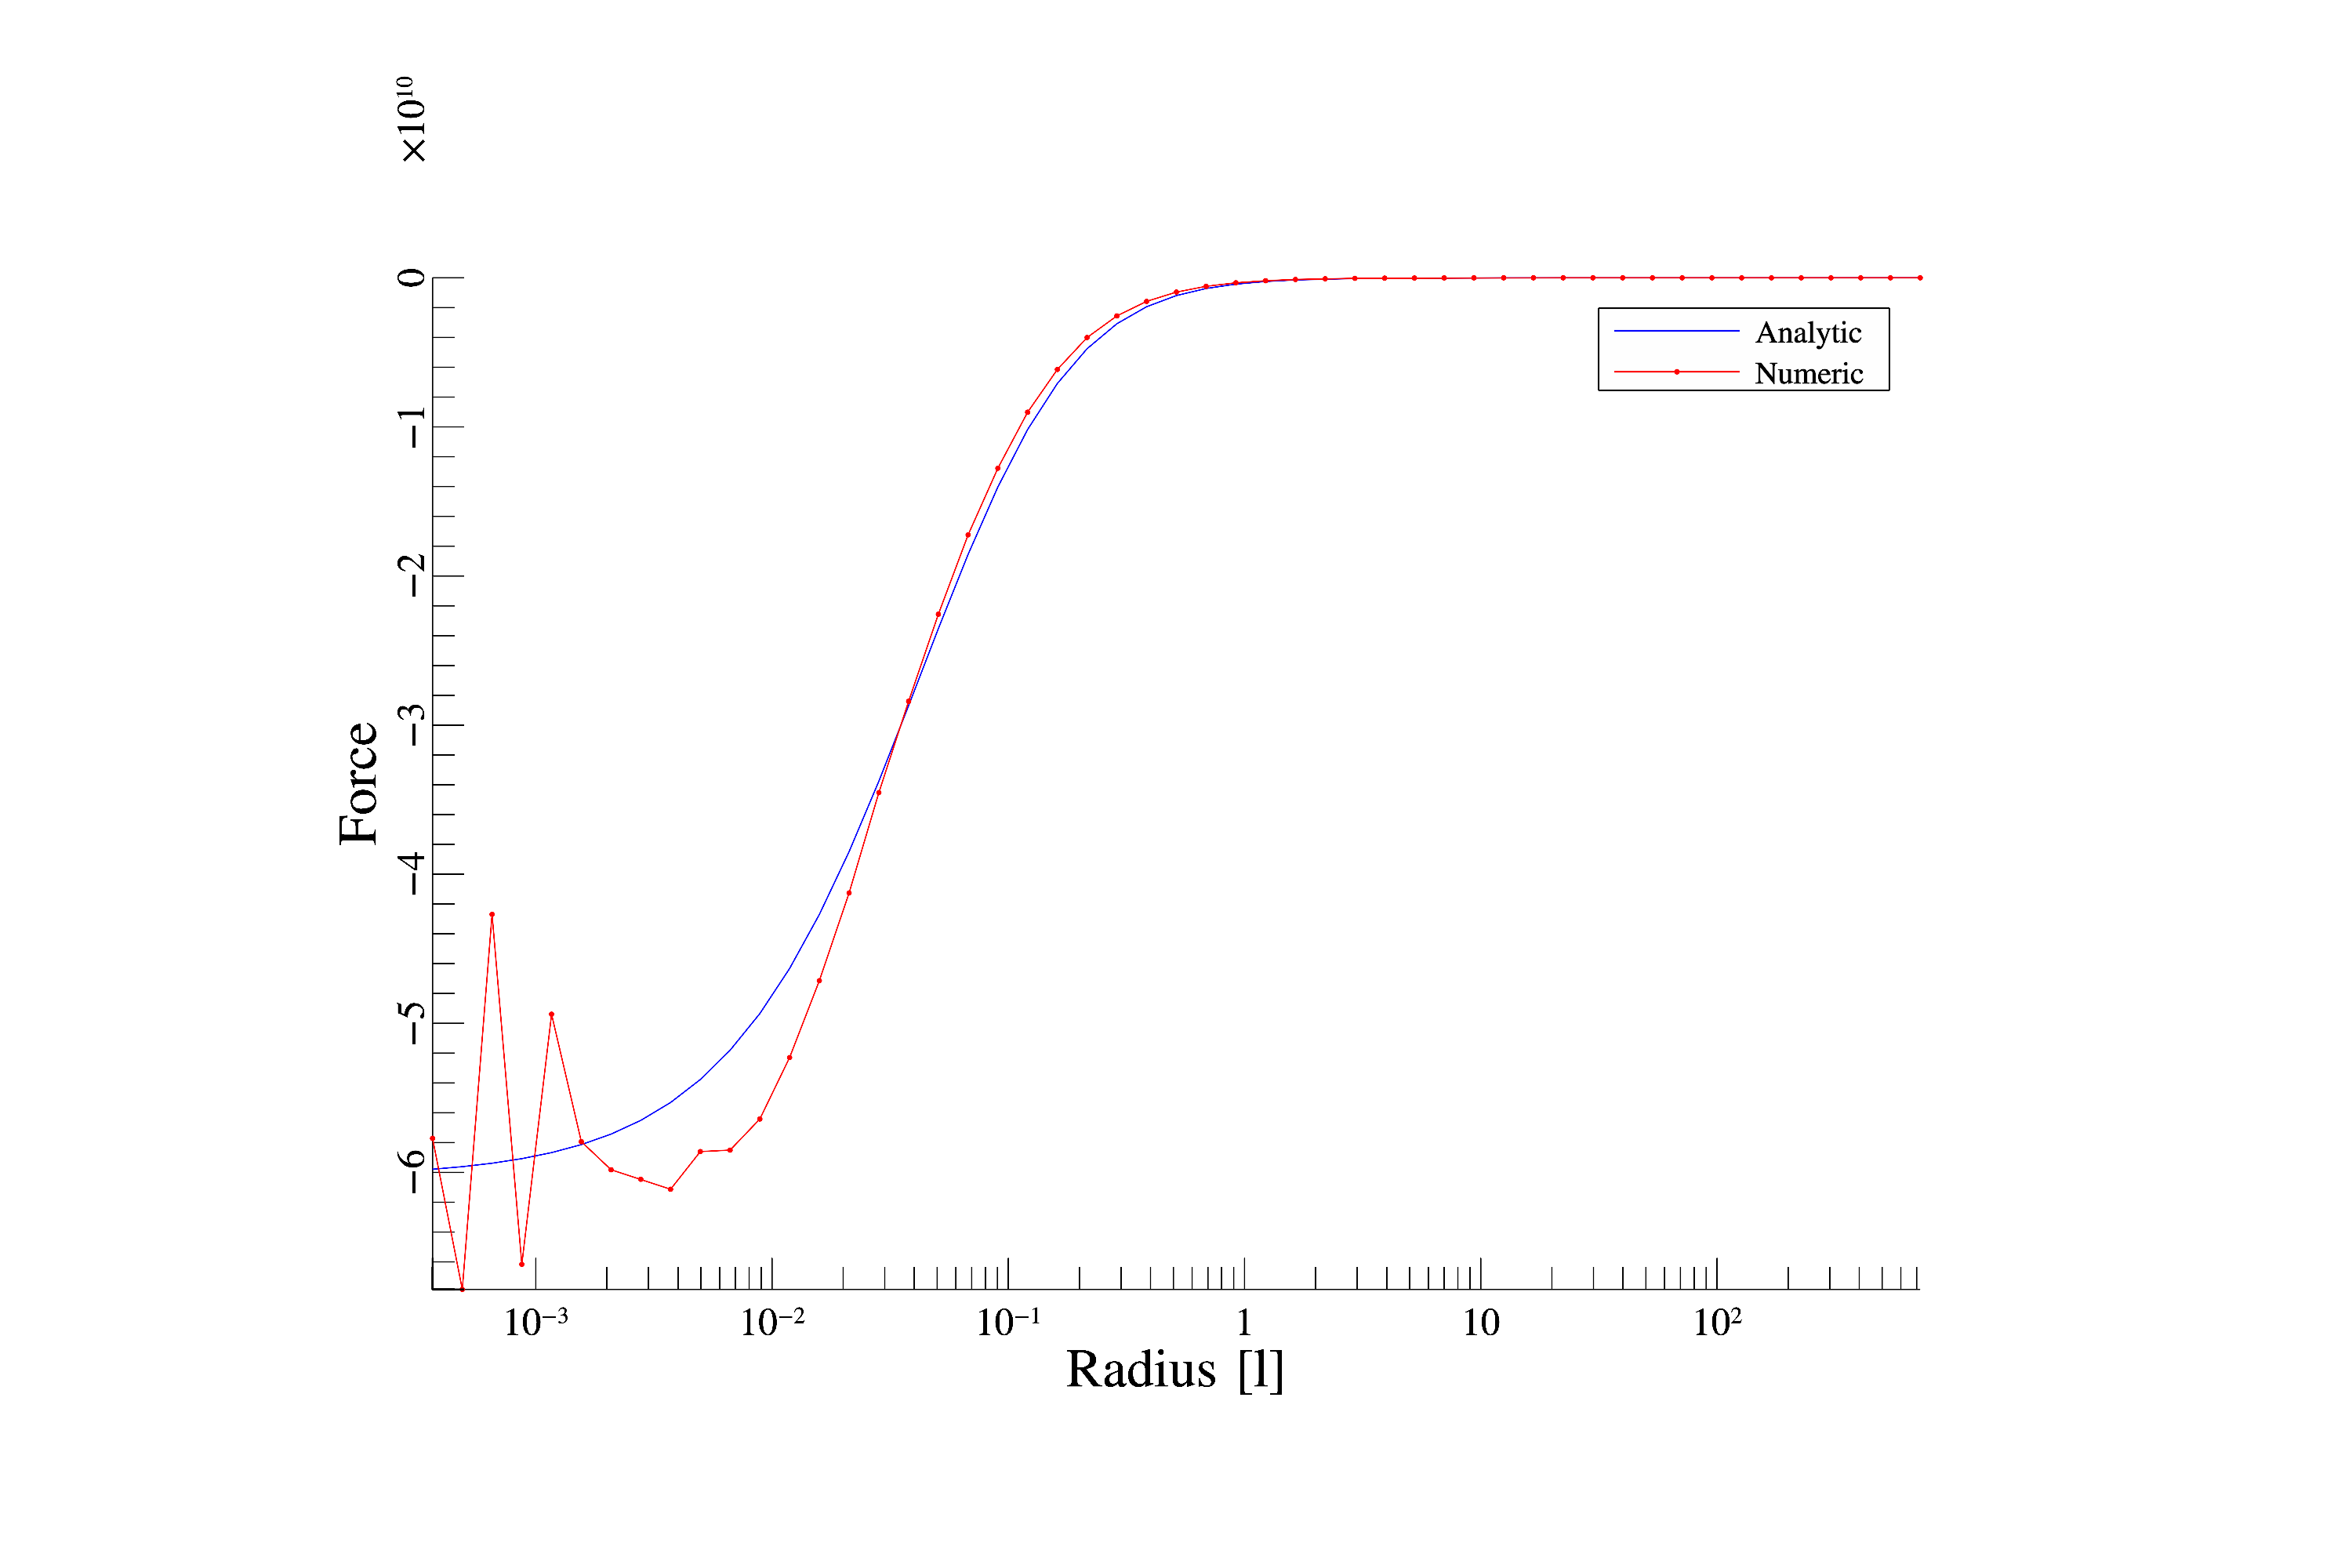
\includegraphics[width=0.95\textwidth]{figures/plots/forces_d_128.png}
\end{frame}

\begin{frame}{Relaxation Timescale}
	% Increasing the gravitational softening above the interparticle separation alters the close encounters between particles.
	% It reduces the impact of these encounters on particle trajectories.
	% As a result, the energy exchange during encounters becomes less efficient. This would typically lead to an 
	% increase in the relaxation timescale, because it would take longer for the system to reach equilibrium due to
	% the less frequent and less effective energy exchanges.

	% Although, since the relaxation calculation is purely analytical, there is no real correlation between the
	% values.

	\begin{equation}
		v_c = \sqrt{GM(R_{hm})/R_{hm}}
	\end{equation}
	\begin{equation}
		t_{cross} = \frac{R_{hm}}{v_c}
	\end{equation}
	\begin{equation}
		t_{relax} = \frac{N}{8\ln{N}}t_{cross}
	\end{equation}

	\bigskip
	Using:
	\begin{itemize}
		\item $G = \SI{4.3009172706e-3}{\parsec.\solarmass^{-1}.(\kilo\metre\per\second)^2}$
		\item $m = \SI{92.4259}{\solarmass}$
	\end{itemize} \bigskip

	Crossing Timescale: $898.302\ yr$ \\
	Relaxation Timescale: $0.520\ Myr$

\end{frame}
